\subsection{The deuteron}
\label{sub:deuteron}


While the first applications of NQS to many-body problems date to 2017--18~\cite{carleo_solving_2017,Saito2017,Saito2018}, the first application to a nuclear system arrived in 2020 with Ref.~\cite{keeble_machine_2020}. That work presented a proof-of-principle calculation of the deuteron, the only bound state of a neutron and a proton. The setup was deliberately minimal, allowing the authors to focus on the capabilities of the NQS framework rather than on details of the ansatz architecture.

\begin{figure}[!b]
\centering
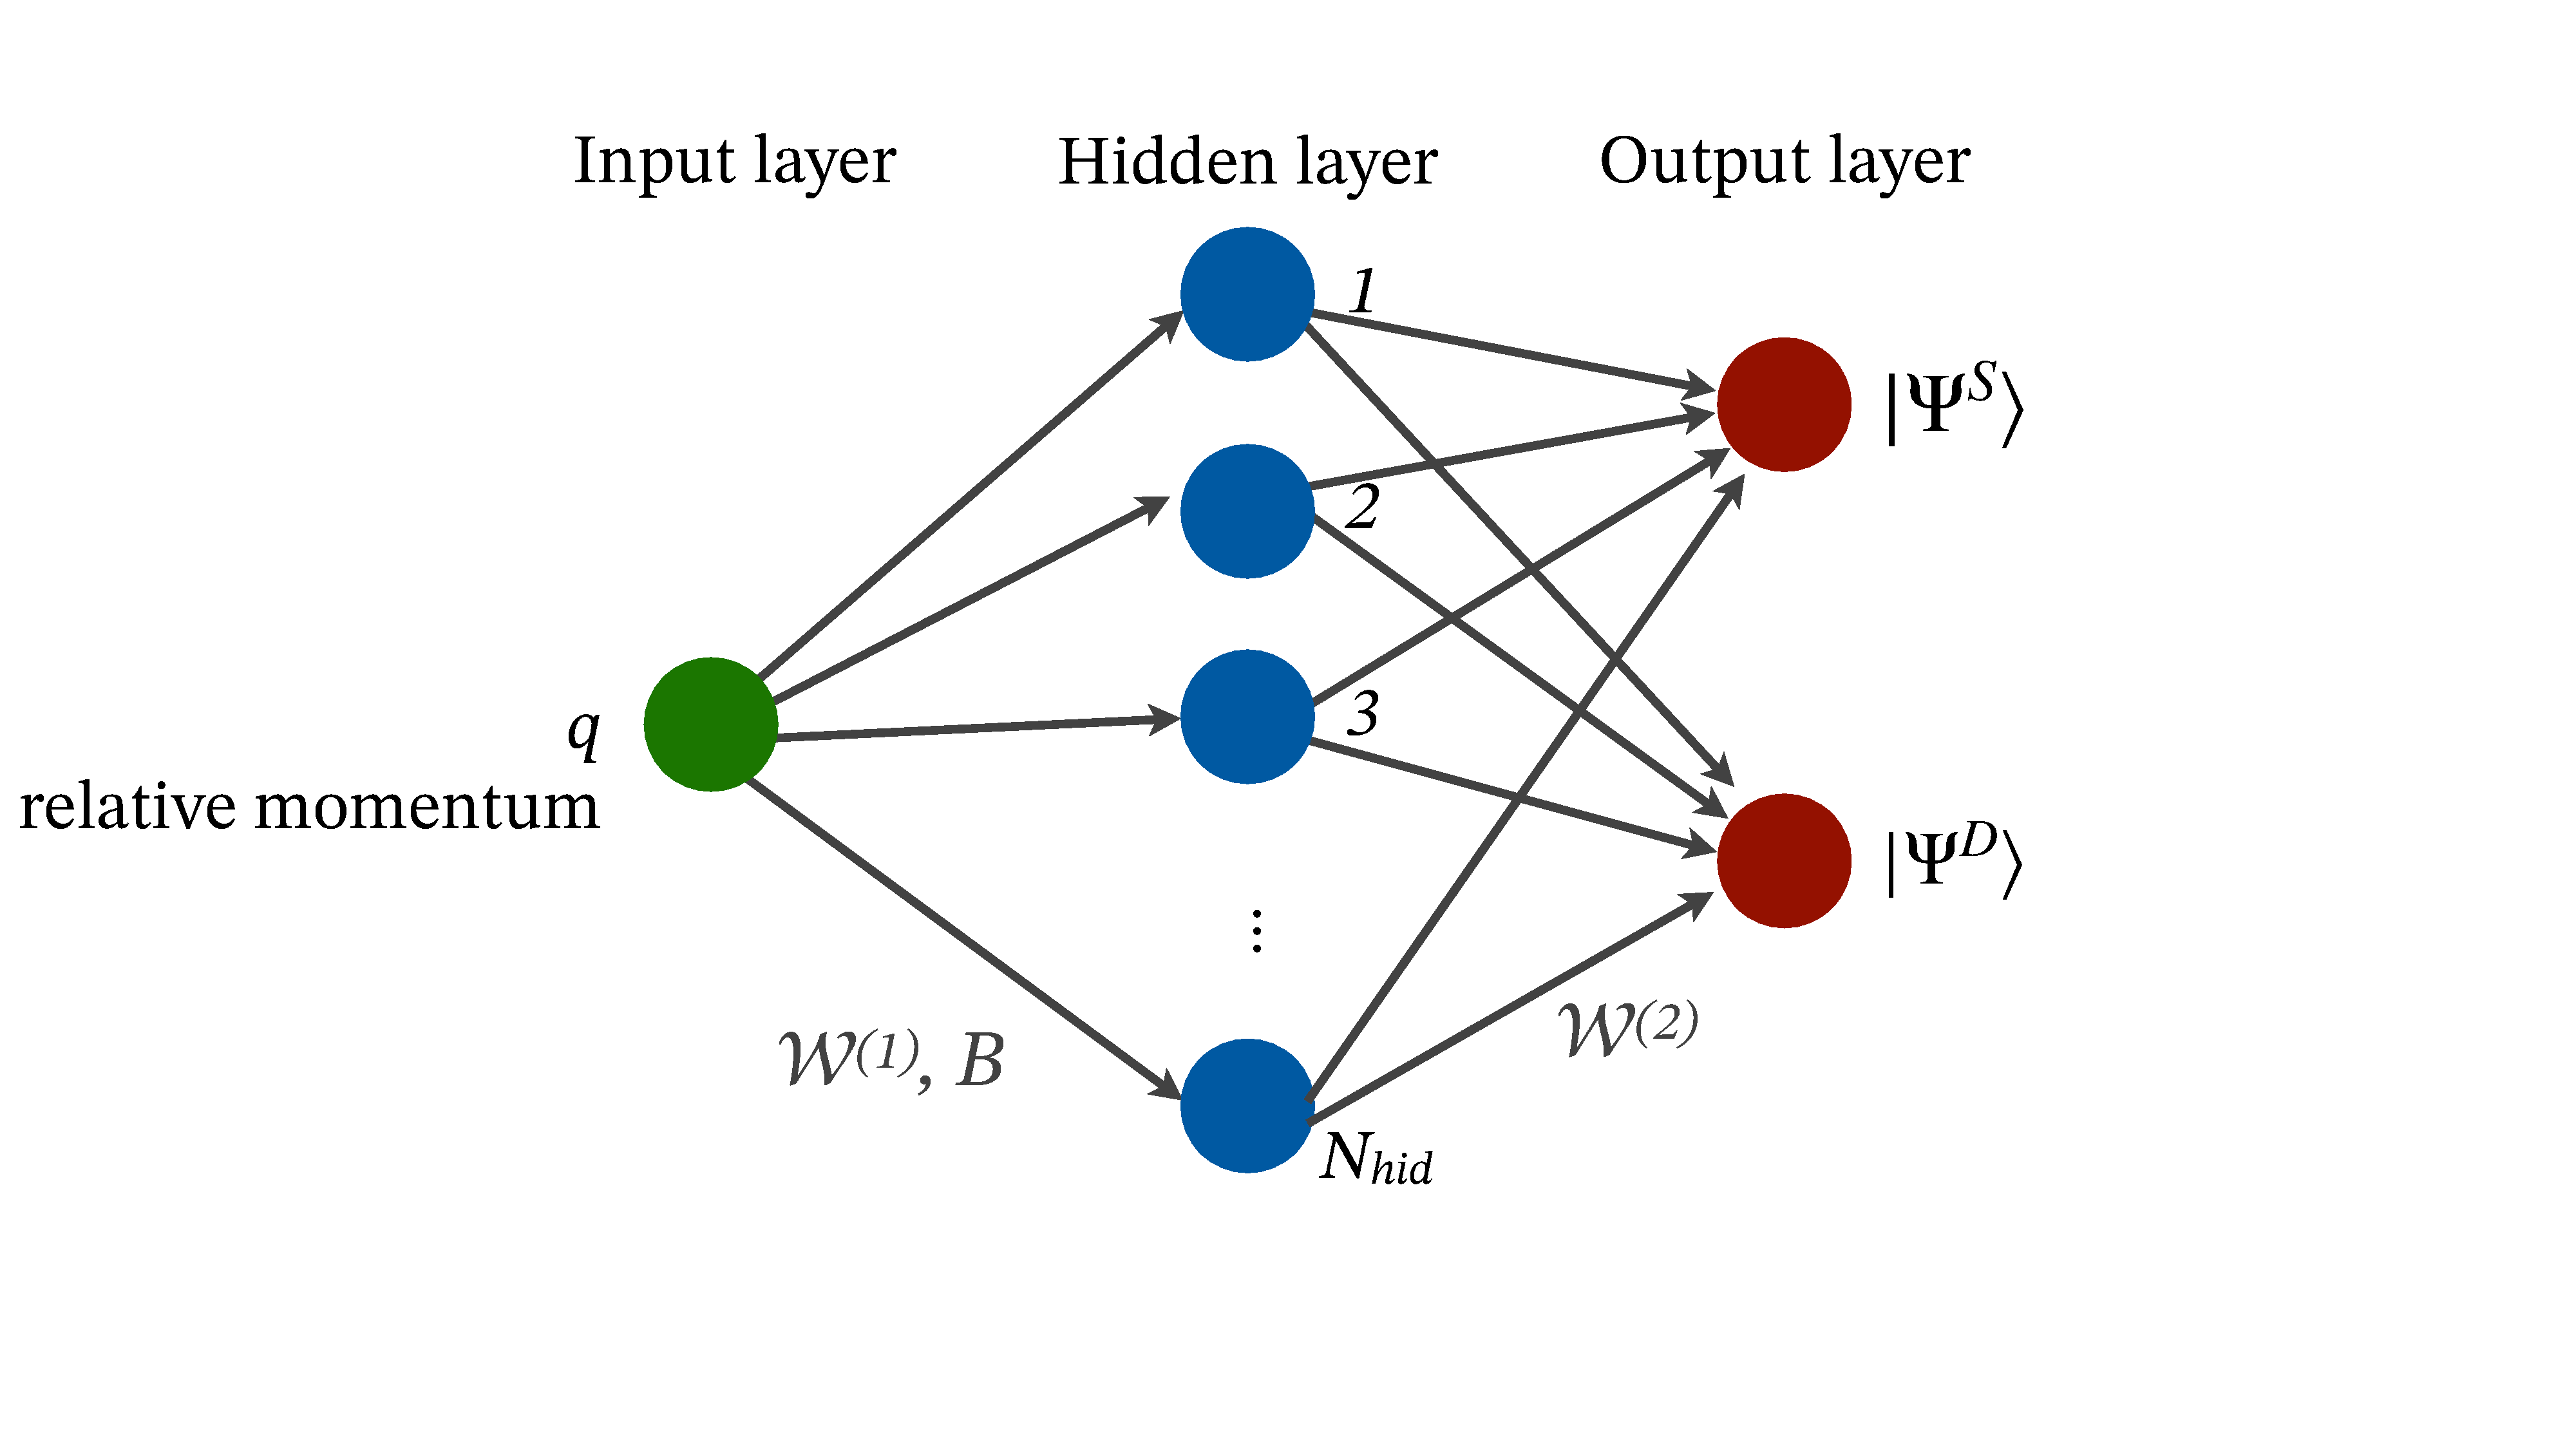
\includegraphics[width=0.7\linewidth]{figures/deuteron/arch_0.pdf}
\caption{\label{fig:NN_deuteron} 
Feed-forward neural network architecture used in Ref.~\cite{keeble_machine_2020}. The input is a single value of relative momentum, $q$, and the wave functions are modeled in terms of a minimal single-layer network with $N_\text{hid}$ nodes. The ansatz has two outputs, one for the $S$ and one for the $D$ state.
}  
\end{figure}

Because nucleon--nucleon interactions are naturally formulated in momentum space~\cite{Epelbaum:2009rkz}, and many existing numerical routines operate in this representation, the initial application was carried out in momentum space. In this basis, the two-body problem factorizes into a center-of-mass component and a relative component, with the former being irrelevant for the bound-state problem. The relative component is characterized by the relative momentum $q$ between the neutron and the proton. An additional practical advantage of working in momentum space is that no derivatives associated with the kinetic energy operator are required. In this formulation, the bound-state wave function can be decomposed into partial waves of definite orbital angular momentum.
The deuteron exhibits a known quadrupole deformation~\cite{Epelbaum:2009rkz}, implying that its wave function contains both a relative orbital angular momentum $L=0$ component, denoted $\ket{\Psi^S}$, and an $L=2$ component, denoted $\ket{\Psi^D}$.


With these nuclear properties in mind, a minimal ansatz for the deuteron wave function was chosen, as shown in Fig.~\ref{fig:NN_deuteron}. The ansatz consists of a simple MLP with one input (the relative momentum $q$) and two outputs (the two components $\ket{\Psi^{S,D}}$). The first layer included a set of weights ${\bf \mathcal{W}}^{(1)}$ and biases $\mathbf{b}$, whereas the second layer did not incorporate any bias. The network contained $N_\text{hid}$ hidden nodes and was assumed to be fully connected, as indicated in Fig.~\ref{fig:NN_deuteron}. The wave-function ansatz has the form
\begin{align}
    \psi_{\textrm{ANN}}^L (q) =  \sum_{i=1}^{N_\text{hid}} \mathcal{W}^{(2)}_{i,L} \, \sigma \left( \mathcal{W}^{(1)}_{i} q + b_{i} \right) \, ,
    \label{eq:wfANNdeuteron}
\end{align}
where $\sigma(x)$ denotes the chosen activation function. Since the deuteron wave function is a smooth, continuous function of $q$, it is natural to employ continuous activation functions in this case. The initial exploration of Ref.~\cite{keeble_machine_2020} considered both sigmoid and softplus functions.
 


The one-dimensional nature of the problem in relative momentum coordinates allows the total energy to be evaluated straightforwardly by quadrature. For example, the kinetic energy expectation value is approximated as
\begin{align}
    \braket{K} = \sum_L 
    \int_0^\infty dq \, q^2 
    \frac{\hbar^2 q^2}{\mu} | \Psi^L(q) |^2
    \approx 
    \sum_L \sum_{i=1}^{N_q} \omega_i \, q_i^2 
    \frac{\hbar^2 q_i^2}{\mu} | \Psi^L(q_i) |^2 \, ,
    \label{eq:kinetic}
\end{align}
where $\mu = m_n m_p /(m_n + m_p)$ is the reduced mass of the $np$ system. 
A set of $N_q = 64$ Gauss--Legendre quadrature points, tangentially transformed to extend up to $k_\textrm{max} = 500$ fm$^{-1}$, was sufficient to obtain accurate results. The same quadrature scheme can be used to evaluate the potential energy.
This initial study employed the N3LO Entem--Machleidt interaction~\cite{Entem2003}, although in principle any other interaction could be used. The quadrature-discretized Hamiltonian can of course be diagonalized directly, providing an exact benchmark on the same footing as the NQS simulation.

%Minimization - RMSprop
With this quadrature set up, the calculation of the energy is rather straightforward. The original set-up employed a pre-training step to pre-optimize the shape of the ansatz in Eq.~\eqref{eq:wfANNdeuteron} to physically sound values. This step is not necessary, but helps accelerate the optimization procedure~\cite{rozalen_sarmiento_machine_2024}. 
After the pre-training, the energy minimization was performed over $250,000$ steps employing RMSprop~\cite{hinton_lecture_2012} as the optimizer of choice. 
%At the stage, the energy is typically converged to within $2-3 \%$ of the benchmark. 

\begin{figure}
\centering
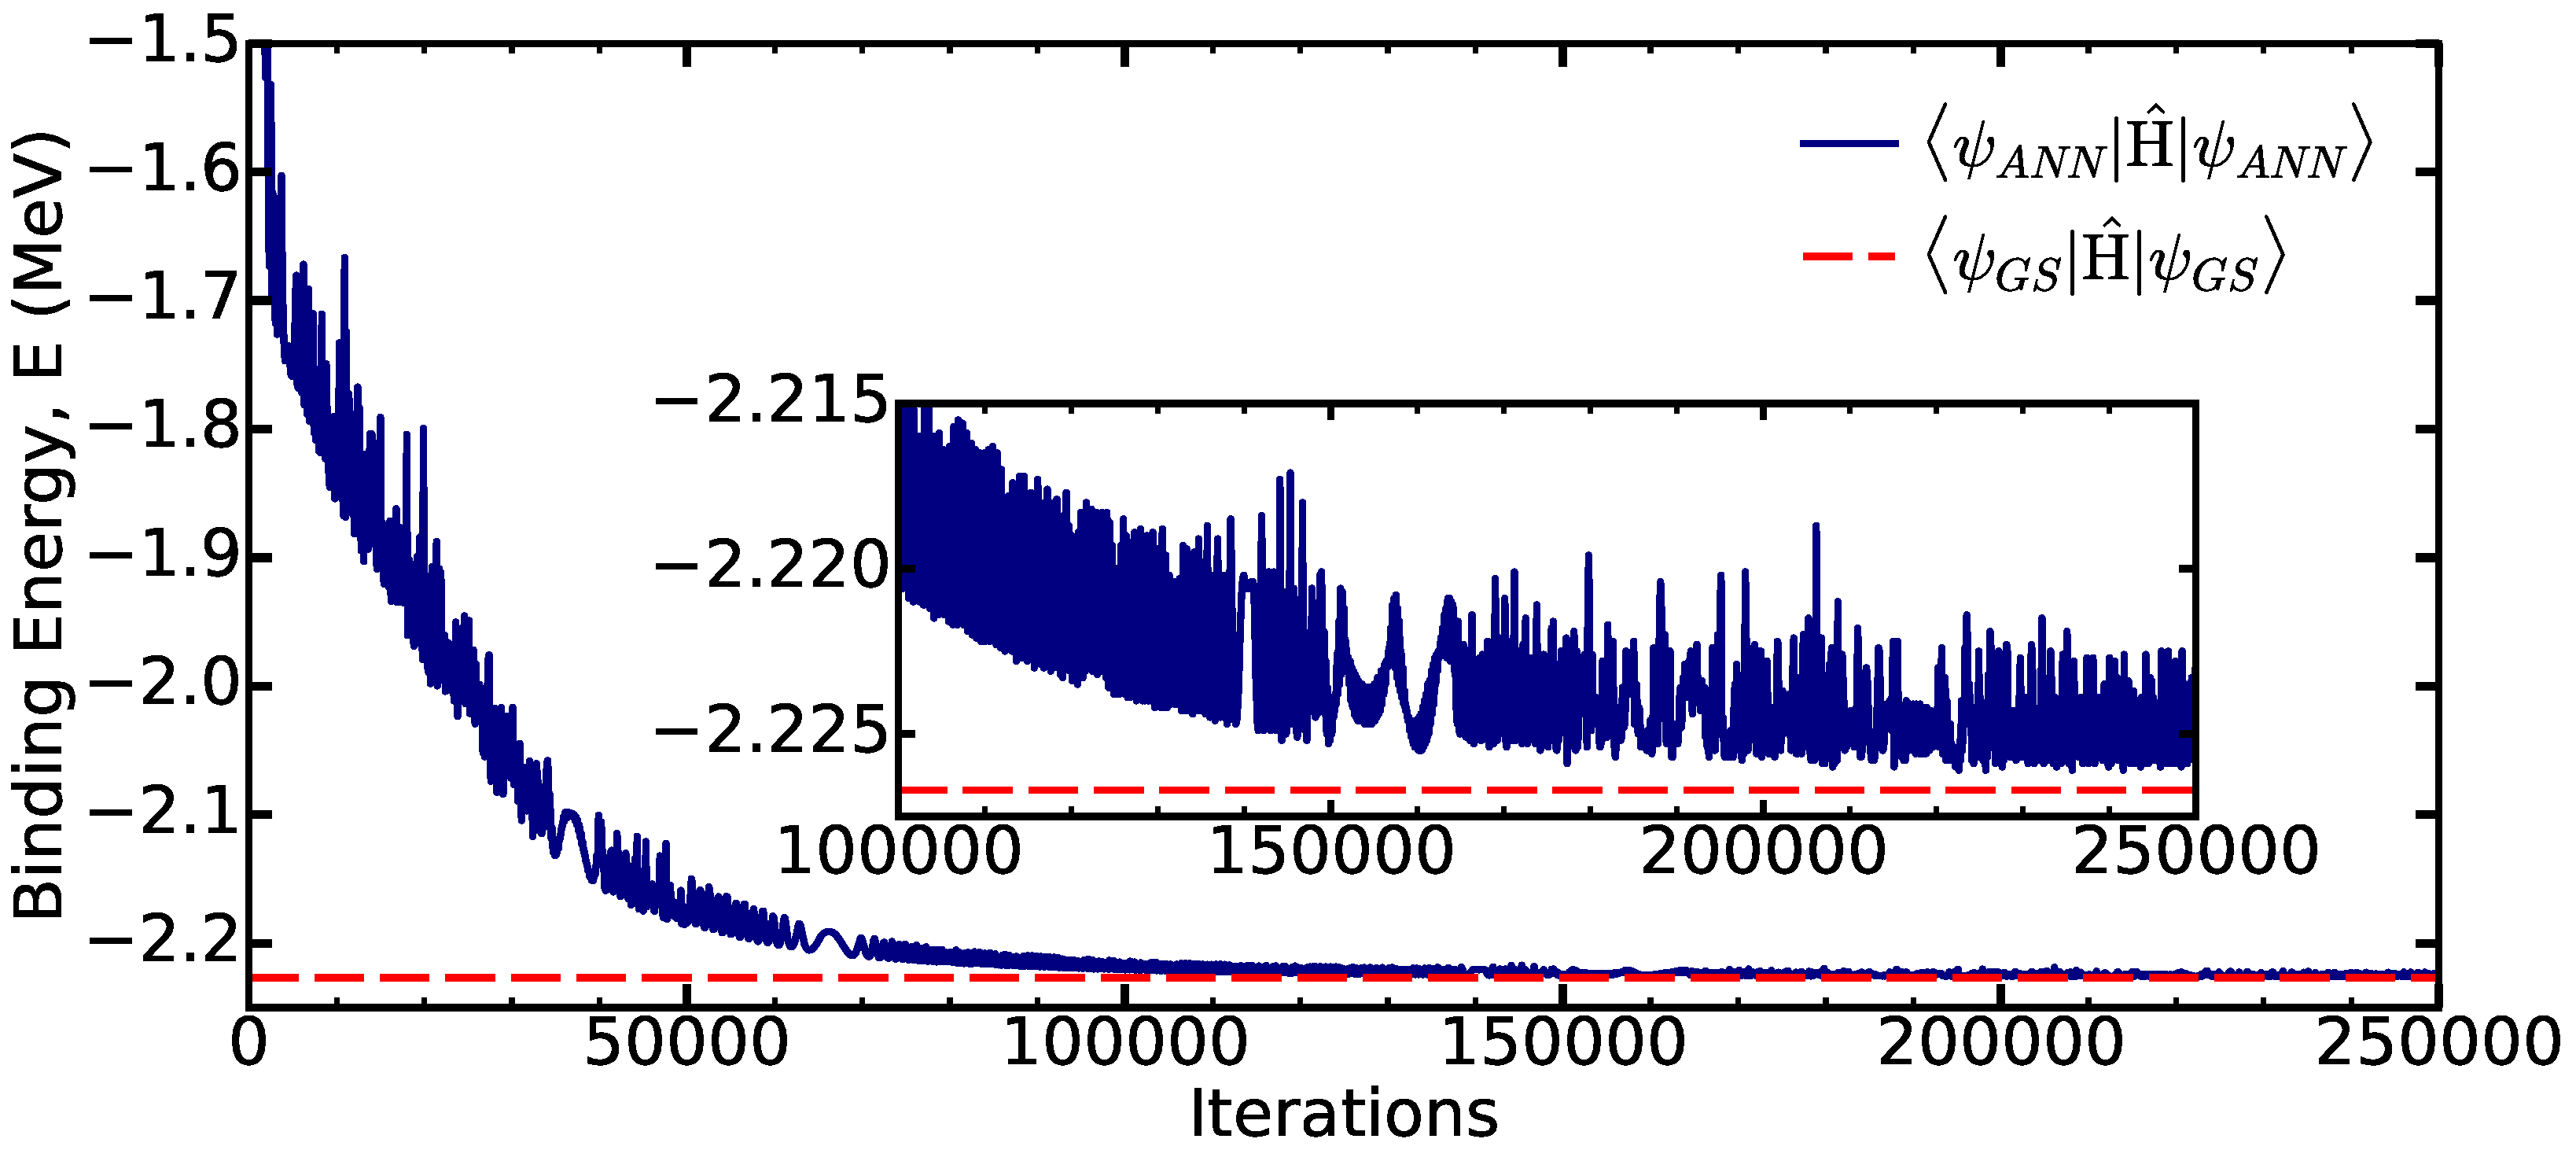
\includegraphics[width=0.7\linewidth]{figures/deuteron/Energy_vs_Epochs_Nhid_10_softplus_RMSprop_run01.pdf}
\caption{\label{fig:energy_deuteron_minimisation} 
Deuteron binding energy as a function of iteration number for a network with 
$N_\text{hid} = 10$ nodes and a softplus activation function~\cite{keeble_machine_2020}.}  
\end{figure}

A typical minimization curve for the case with $N_\text{hid}=10$ is shown in Fig.~\ref{fig:energy_deuteron_minimisation}. For this very simple architecture, the energy converged to $1 \%$ within a few tens of thousands of iterations. 
After around $150,000$ iterations, the energy is very close to the minimum, but oscillates above the actual benchmark minimum within $3-4$ eV of the exact result. 
This minimal set-up already provides an excellent reproduction of the exact wave function and physical properties of the deuteron~\cite{keeble_machine_2020}.

To address systematic errors in the NQS method as opposed to specific minimisations, the analysis of Refs.~\cite{keeble_machine_2020} and \cite{rozalen_sarmiento_machine_2024} focused on the characterization of uncertainties. Simulations of the deuteron were run for different numbers of hidden nodes, $N_\text{hid}$. Results of these numerical experiments for the simple architecture of Eq.~\eqref{eq:wfANNdeuteron} are presented in Fig.~\ref{fig:deuteron_energies}~\cite{rozalen_sarmiento_machine_2024}. 
%We refer the interested reader to Ref.~\cite{rozalen_sarmiento_machine_2024} for information on more sophisticated architectures. 
Two different sets of uncertainties were identified to characterize the NQS minimization generally (as opposed to a minimization-by-minimization basis). First, different initializations of the network lead to different final results after $250,000$ iterations. This uncertainty can be assessed by running the minimization process $20$ times and computing the associated standard deviation. This out-of-sample uncertainty is represented in dark bands in the top panel of Fig.~\ref{fig:deuteron_energies}. We stress that this uncertainty amounts to only a fraction of a keV in energy and that it is rather independent of the number of nodes. Moreover, the fidelity, $F$, between the ansatz at the end of minimization and the corresponding exact benchmark is given in the bottom panel of Fig.~\ref{fig:deuteron_energies}. We represent the fidelities of both the $S-$ and the $D-$states. Again, out-of-sample uncertainties, represented by dark bands, are very small for fidelities~\cite{keeble_machine_2020}. 


%Fig energies
As illustrated in Fig.~\ref{fig:energy_deuteron_minimisation},  even at the end of a full minimization, the results still show some residual oscillations. 
These oscillations are typically within a few keV of the total energy and are hence larger than the out-of-sample uncertainty. In this context, Ref.~\cite{rozalen_sarmiento_machine_2024} looked into these post-training oscillation amplitudes as an additional source of uncertainty that is associated not so much to minimization instances, but rather to the minimization process itself. To characterize this uncertainty, the model was minimized initially and then evolved for $300$ final iterations. The number of these post-evolution epochs is small, to guarantee that mean energy values do not improve, but also large enough to observe periodicity in the oscillations. Upper and lower values of these oscillations were recorded for $20$ different minimization instances, and their average values are shown as the light bands in Fig.~\ref{fig:deuteron_energies}. 

These results clearly indicate that  oscillation errors at the end of the minimization dominate over any out-of-sample uncertainties. Moreover, these uncertainties show a decreasing trend with $N_\text{hid}$. Whereas for $N_\text{hid}=2$ the post-evolution uncertainty in the energy is of the order of $2.5$ keV, at $N_\text{hid}=100$ this falls just below $1$ keV. A similar decrease in post-evolution uncertainty is observed in the fidelities of the bottom panel. In this case, the fidelity of the $D-$state presents a much larger uncertainty. 

\begin{figure}
\centering
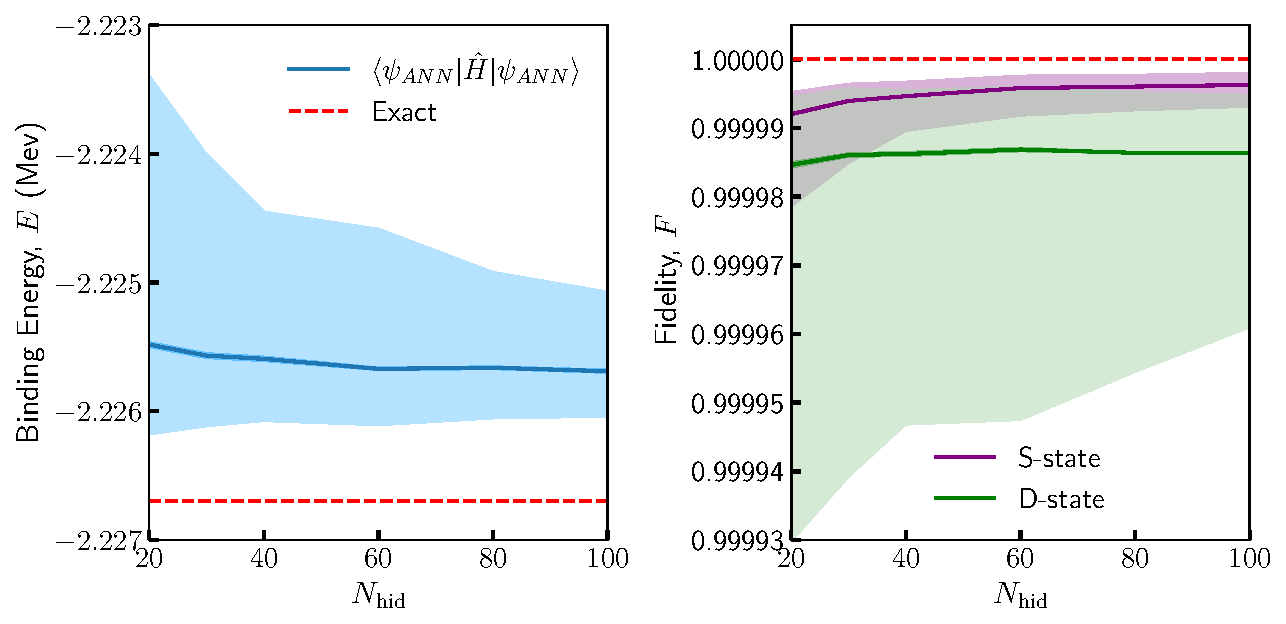
\includegraphics[width=0.8\linewidth]{figures/deuteron/deuteron_1sc_master_plot.pdf}
\caption{\label{fig:deuteron_energies} 
Binding energy of the deuteron (left panel) and fidelity $\mathcal{F}$ (right panel) as a function of the number of hidden layer nodes, $N_\text{hid}$ from Ref.~\cite{rozalen_sarmiento_machine_2024}. See main text for an explanation of the error bands. Horizontal (dashed) lines show the benchmark result. 
}  
\end{figure}

%Fig wave functions

The high fidelity shown in Fig.~\ref{fig:deuteron_energies} indicates a strong level of agreement between the exact wave function and the NQS ansatz. This agreement is illustrated more explicitly in Fig.~\ref{fig:deuteron_wave functions}, which displays the $S$- (left panel) and $D$-wave (right panel) components as functions of momentum for minimizations with $N_\text{hid}=10$~\cite{keeble_machine_2020}. The solid (red) lines correspond to the benchmark exact solution, while the dashed (blue) and dotted (green) lines show the results of averaging 50 independent minimizations using sigmoid and softplus activation functions, respectively.

The agreement is excellent across nearly all momenta, with small deviations appearing near the origin, $q \approx 0$ fm$^{-1}$. Because the wave functions are spherically symmetric, the energy functional includes a $q^2$ factor in the integration measure. As a result, the region near $q=0$ contributes very little to the cost function, leaving the wave function weakly constrained there. A simple network with $N_\text{hid}=10$ has limited flexibility to adjust its behavior in this region. As $N_\text{hid}$ increases, however, additional flexibility tends to manifest primarily near the origin, where the weak energetic penalty may allow for large variations in shape, including non-physical behaviors~\cite{keeble_machine_2020}.


\begin{figure}
\centering
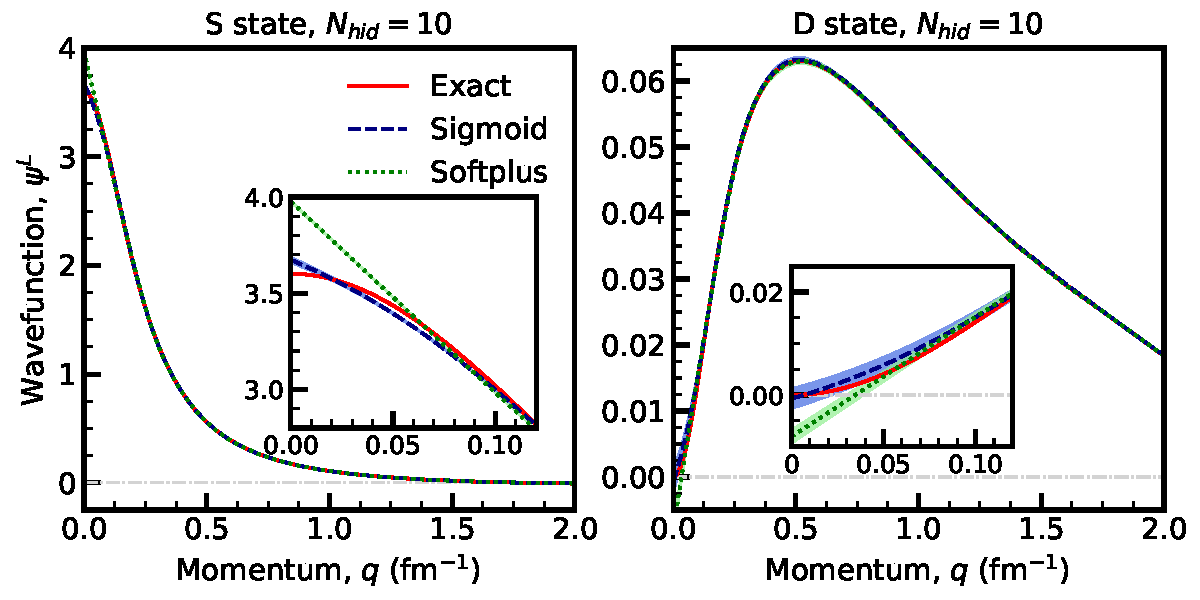
\includegraphics[width=0.75\linewidth]{figures/deuteron/compare_wavefunctions_Nhid10.pdf}
\caption{\label{fig:deuteron_wave functions} 
Left (right) panel: the $S$ ($D$) state wave function as a function of momentum, taken from Ref.~\cite{keeble_machine_2020}. The benchmark exact solutions (solid lines) are compared to the feed-forward ansatz with $N_\text{hid}=10$ using sigmoid (dashed) and softplus (dotted) activation functions. The shaded bands indicate the standard deviation over 50 different initialization runs.
}  
\end{figure}

%More elaborate architectures
% Acceptance rate
While our discussion has focused on the simple architecture of Eq.~\eqref{eq:wfANNdeuteron}, Ref.~\cite{rozalen_sarmiento_machine_2024} presents an extensive analysis of more elaborate architectural extensions. These include separate, independent branches for the $S$ and $D$ channels, as well as deeper, multi-layer networks.
Adopting these more complex architectures leads to two main consequences. First, the fraction of models that converge to an acceptable energy range, $E \in (-2.220, -2.227)$ MeV, is significantly reduced. Whereas the simple one-layer MLP achieves a $100\%$ success rate for nearly all values of $N_\text{hid}$, the acceptance rates of more complex architectures depend strongly on $N_\text{hid}$ and range from $1\%$ to $90\%$~\cite{rozalen_sarmiento_machine_2024}. Second, more elaborate architectures exhibit substantially larger post-training uncertainties,  with a pronounced dependence on $N_\text{hid}$. In some cases, indications of overfitting are also observed. Although understanding the internal behavior of NQS models is not easy, the systematic error analysis and architectural comparisons performed for the deuteron provide a useful starting point for probing these issues in nuclear systems.

\subsection{Atomic nuclei}
\label{sub:nuclei}

\subsubsection[Nuclei with up to A=6 nucleons]{Nuclei with up to A=6 nucleons}
The first application of VMC methods based on NQS to the nuclear many-body problem~\cite{adams_variational_2021} computed the ground-state energies and single-particle densities of $^2$H, $^3$H, and $^4$He. It is worth noting that the LO pionless-EFT Hamiltonian used in that work differs slightly from the one discussed in Sec.~\ref{sec:nmbp}. Specifically, the NN interaction is
\begin{equation}
v_{\mathrm{LO}}^{\mathrm{CI}}(r_{ij}) = \bigl(C_1 + C_2 \sigma_{ij}\bigr)
e^{-r_{ij}^2 \Lambda^2 / 4},
\label{eq:v_nn_contessi}
\end{equation}
where, following Ref.~\cite{kirscher_spectra_2015}, the low-energy constants $C_1$ and $C_2$ are fitted to the deuteron binding energy and the neutron–neutron scattering length. The 3N force is taken as
\begin{equation}
V_{ijk} = D_0 \sum_{\mathrm{cyc}}
e^{-(r_{ik}^2 + r_{ij}^2)\Lambda^2/4},
\end{equation}
with $D_0$ fixed by the $^3$H ground-state energy.

\begin{table}[!b]
\begin{center}
\begin{tabular}{ c | c | c c c c }
\hline
\hline
& $\Lambda$ & SJ  &  Spline & GFMC\\
\hline
\multirow{2}{*}{$^2$H } & $4$ fm$^{-1}$ & $-2.224(1)$  &   $-2.223(1)$  & $-2.224(1)$ \\
& $6$ fm$^{-1}$ & $-2.224(4)$  &   $-2.220(1)$  & $-2.225(1)$ \\
\hline
\multirow{2}{*}{$^3$H } & $4$ fm$^{-1}$ & $-8.26(1)$  &   $-7.80(1)$  & $-8.38(2)$ \\
& $6$ fm$^{-1}$ & $-8.27(1)$  &   $-7.74(1)$  & $-8.38(2)$ \\
\hline
\multirow{2}{*}{$^4$He } & $4$ fm$^{-1}$ & $-23.30(2)$  &   $-22.54(1)$  & $-23.62(3)$ \\
& $6$ fm$^{-1}$ & $-24.47(3)$  &   $-23.44(2)$  & $-25.06(3)$ \\
\hline
\end{tabular}
\caption{(From Ref.~\cite{adams_variational_2021} with permission from the Authors). Ground-state energies in MeV of the $^2$H, $^3$H, and $^4$He for the LO pionless-EFT Hamiltonian for $\Lambda = 4$ fm$^{-1}$ and $\Lambda = 6$ fm$^{-1}$. Numbers in parentheses indicate the statistical errors on the last digit.}
\label{tab:2h}
\end{center}
\end{table}

Reference~\cite{adams_variational_2021} employed the SJ wave-function ansatz of Eq.~\eqref{eq:SJ}, together with the real-valued Jastrow factor of Eq.~\eqref{eq:jastrow_tanh}. In this construction, the Deep Sets architecture (see Section~\ref{sec:deep_learning}) uses the single-particle sum aggregation of Eq.~\eqref{eq:deep_sets_single}. Table~\ref{tab:2h}, adapted from Ref.~\cite{adams_variational_2021}, reports the ground-state energies of $^2$H, $^3$H, and $^4$He. The SJ results are benchmarked against VMC calculations based on spline parameterizations of the two- and three-body spin–isospin–independent Jastrow functions~\cite{contessi_ground-state_2017}, as well as against virtually exact GFMC results.
All three methods yield statistically consistent energies for $^2$H, demonstrating that the SJ ansatz is flexible enough to accurately represent the deuteron ground state. This agrees with the findings of Ref.~\cite{keeble_machine_2020}, discussed in Section~\ref{sub:deuteron}. Since the LO pionless-EFT Hamiltonian lacks tensor and spin–orbit components, the SJ ansatz without backflow is in fact exact for this system.
For $^3$H, the neural SJ ansatz provides an improvement of about $0.5$~MeV over conventional VMC for both $\Lambda = 4$~fm$^{-1}$ and $6$~fm$^{-1}$. The GFMC energies are roughly $0.1$~MeV more bound than the SJ ones. As noted in Ref.~\cite{adams_variational_2021}, this residual difference originates from spin-dependent correlations that are automatically generated in GFMC imaginary-time evolution but are only partially encoded in the Jastrow factor of Eq.~\eqref{eq:jastrow_tanh}. These correlations modify the nodal structure of the wave function, which the SJ architecture cannot recover without incorporating backflow transformations.
A similar trend is observed for $^4$He: the SJ wave functions outperform the conventional VMC ones, improving the energies by about $0.8$~MeV and $1.0$~MeV for $\Lambda = 4$~fm$^{-1}$ and $6$~fm$^{-1}$, respectively. The remaining discrepancies with GFMC again reflect missing spin–isospin–dependent correlations in the SJ ansatz.



 
\begin{figure}[!htb]
\centering
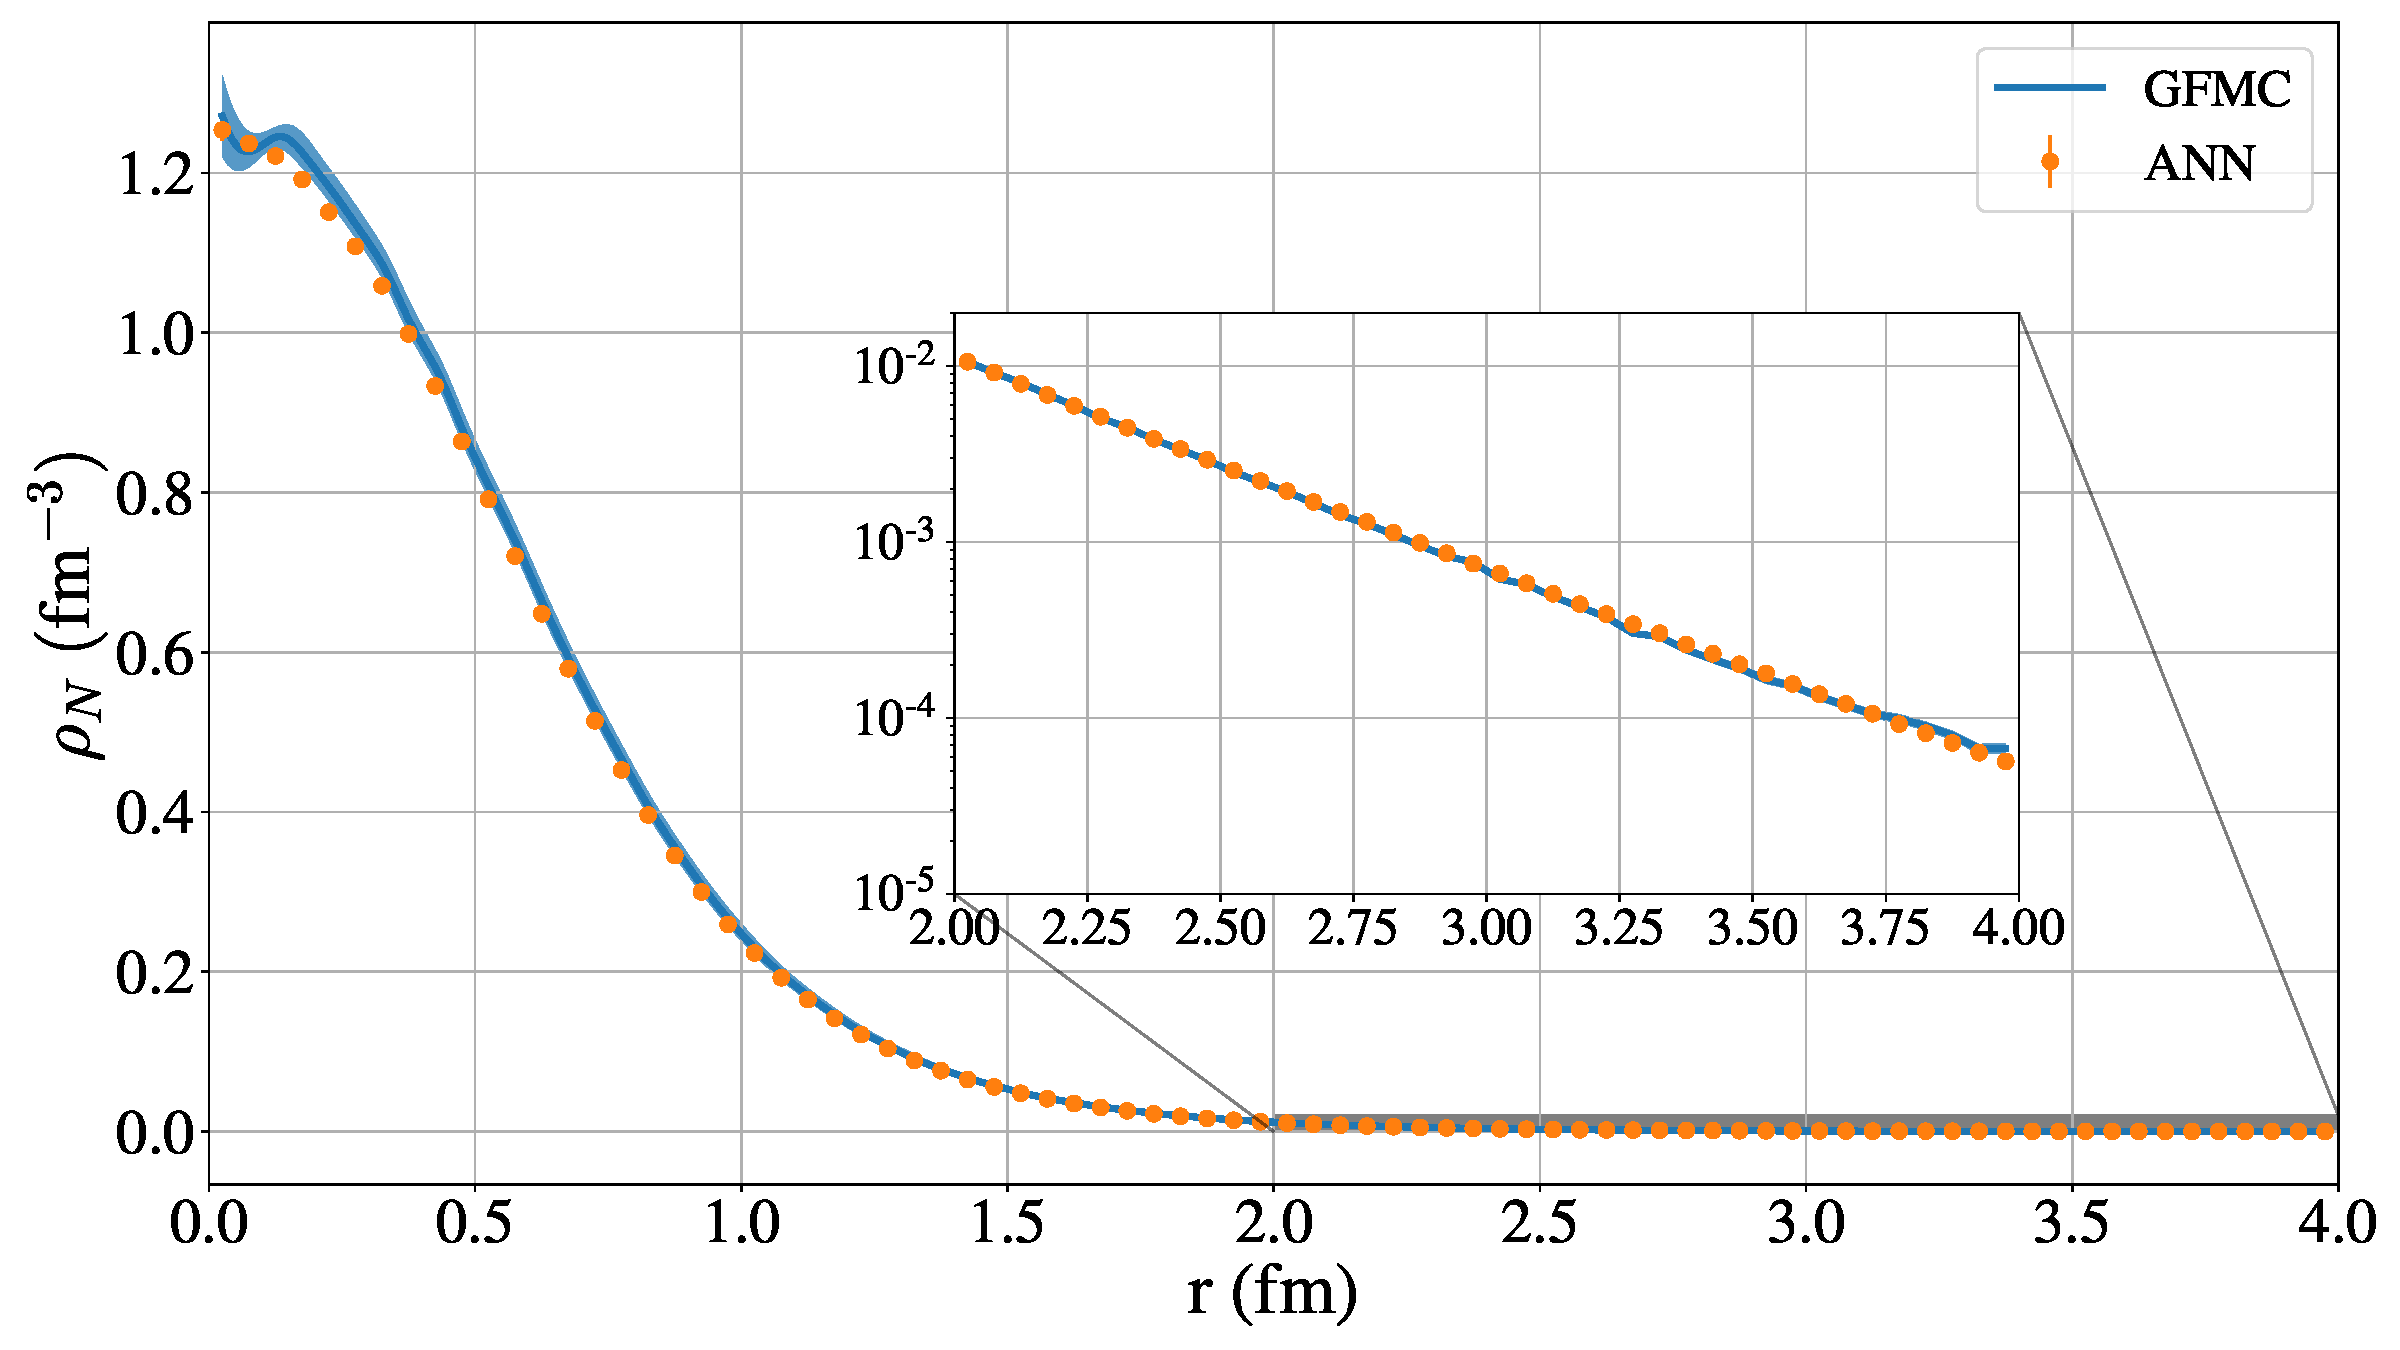
\includegraphics[width=0.75\columnwidth]{figures/applications/rho_4he.pdf}
\caption{(From Ref.~\cite{adams_variational_2021}, with permission from the Authors) Point-nucleon densities of $^4$He (lower panel) for the LO pionless-EFT Hamiltonian with $\Lambda =4$ fm$^{-1}$. The solid points and the shaded area represent the SJ and GFMC results, respectively.}
\label{fig:rho_4he}
\end{figure}

To further elucidate the quality of the ANN wave function, we consider the point-nucleon density
\begin{align}
	\rho_{N}(r) &=\frac{1}{4\pi r^2}\big\langle\Psi_V \big|\sum_i \mathcal \delta(r-|\mathbf{r}_i^{\rm int}|)\big|\Psi_V \big\rangle\,, 
	\label{eq:rho_N}
\end{align}
which is of interest in a variety of experimental settings~\cite{de_vries_nuclear_1987,angeli_table_2013}. Fig.~\ref{fig:rho_4he} displays $\rho_{N}(r)$ of $^4$He as obtained from the SJ ansatz compared with GFMC calculations, both using as input the LO pionless-EFT Hamiltonian with $\Lambda =4$ fm$^{-1}$. There is an excellent agreement between the two methods, which further corroborates the representative power of the SJ ansatz for the wave functions of $A\leq 4$ nuclei. The SJ and GFMC densities overlap both at short distances and in the slowly-decaying asymptotic exponential tails, highlighted in the insets of Fig.~\ref{fig:rho_4he}. As already noted in Ref.~\cite{adams_variational_2021}, the NQS learns how to compensate for the original Gaussian confining function and reproduce the correct exponential falls off of the nuclear wave function, which is notoriously delicate to obtain within nuclear methods that rely on harmonic-oscillator basis expansions~\cite{caprio_robust_2022,sharaf_comparing_2019}.

Ref.~\cite{Gnech2021} extended the SJ approach to the $^6$Li and $^6$He nuclei, employing the model “o’’ Hamiltonian of Eqs.~\eqref{eq:vNN_LO}-\eqref{eq:o_3NF} with the three-nucleon regulator set to $R_3 = 1.0$~fm. A key technical advance relative to Ref.~\cite{adams_variational_2021} is the use of the linear combination of Slater determinants of Eq.~\eqref{eq:mf} to represent the mean-field component of the open-shell systems $^6$Li and $^6$He. In addition, pairwise inputs were incorporated into the Deep Sets architecture used for the Jastrow factor, as in Eq.~\eqref{eq:deep_sets_pair}. In that work, the SJ energies and charge radii were benchmarked against the highly accurate hyperspherical harmonics (HH) method~\cite{kievsky_high-precision_2008}.

The binding energies and charge radii of $^2$H, $^3$H, $^3$He, $^4$He, $^6$He, and $^6$Li obtained with the VMC method based on the SJ ansatz and with the HH method are listed in Table~\ref{tab:res_NN}. For nuclei with $A \geq 3$, the table separately shows the results computed using the $NN$ interaction alone and those obtained with the full model ``o'' Hamiltonian, which also includes the $3N$ force.

The expectation value of the charge radius is derived from the point-proton radius using the relation:
\begin{align}
	\left\langle r_{\rm ch}^2\right\rangle=
	\left\langle r_{\rm pt}^2\right\rangle+
	\left\langle R_p^2\right\rangle+
	\frac{A-Z}{Z}\left\langle R_n^2\right\rangle+
	\frac{3}{4m_p^2},
	\label{eq:rch}
\end{align}
where $\langle r_{\rm pt}^2\rangle$ is the calculated point-proton radius,
$\langle R_p^2 \rangle = 0.770(9),\mathrm{fm}^2$ is the proton mean-square charge radius,
$\langle R_n^2 \rangle = -0.116(2),\mathrm{fm}^2$ is the neutron mean-square charge radius. Here, consistent with Ref.~\cite{Gnech2021}, we list the 2012 values for these quantities~\cite{beringer_review_2012}. Finally, $(3)/(4m_p^2) \approx 0.033,\mathrm{fm}^2$ is the Darwin–Foldy correction~\cite{friar_nuclear_1997}.
The point-proton radius can be computed as the ground-state expectation value
\begin{align}
	\left\langle r_{\rm pt}^2\right\rangle=\frac{1}{Z}\big\langle\Psi\big|\sum_i P_{p} |\mathbf{r}_i-\mathbf{R}_{\rm cm}|^2\big|\Psi\big\rangle,
\end{align}
where $Z$ is the number of protons and
$P_p = (1 + \tau_{z_i})/2$ projects onto proton states.

\begin{table*}[htb]
\setlength{\tabcolsep}{3.9pt}
\centering
\caption{Ground-state energies and charge radii for selected $A\leq 6$ nuclei obtained from VMC calculations based on the SJ ansatz and HH methods using as input model ``o'' Hamiltonian of Ref.~\cite{schiavilla_two-_2021} with and without the $3N$ force. We report also the experimental binding-energies from
Ref.~\cite{national_nuclear_data_center_nudat_nodate} and the charge radius taken from Refs.~\cite{tiesinga_codata_2021,amroun_3h_1994,morton_nuclear_2006,krauth_measuring_2021,wang_laser_2004,puchalski_ground_2013}.}
\label{tab:res_NN}  
\begin{tabular}{c c c c c c c c}
\hline\hline
\multirow{2}{*}{Nucleus} & \multirow{2}{*}{Potential} & \multicolumn{2}{c}{SJ}               & \multicolumn{2}{c}{HH} & \multicolumn{2}{c}{Exp.}                \\
\noalign{\smallskip}
        &           & $E\,(\rm MeV)$ & $r_{\rm ch}\,(\rm fm)$ & $E\,(\rm MeV)$ & $r_{\rm ch}\,(\rm fm)$ & $E\,(\rm MeV)$ & $r_{\rm ch}\,(\rm fm)$ \\     
\noalign{\smallskip}\hline\noalign{\smallskip}
$^2$H  & $N\!N$ & $-2.242(1)$   & $2.120(5)$ & $-2.242$  & $2.110(2)$ & $-2.225$ & $2.128$\\
\noalign{\smallskip}\hline\noalign{\smallskip}                                                               
\multirow{2}{*}{$^3$H} & $N\!N$& $-9.511(1)$   & $1.658(4)$ & $-9.744$  & $1.656(4)$ & \multirow{2}{*}{$-8.475$} & \multirow{2}{*}{$1.755(86)$}  \\
        & $3N$  & $-8.232(1)$   & $1.750(3)$ & $-8.475$  & $1.747(6)$ & &  \\
\noalign{\smallskip}\hline\noalign{\smallskip}                                                  
\multirow{2}{*}{$^3$He} & $N\!N$& $-8.800(1)$   & $1.845(3)$ & $-9.035$  & $1.848(6)$ & 
\multirow{2}{*}{$-7.718$} & \multirow{2}{*}{$1.964(1)$}  \\
        & $3N$  & $-7.564(1)$   & $1.961(3)$ & $-7.811$  & $1.969(8)$ & & \\
\noalign{\smallskip}\hline\noalign{\smallskip}
\multirow{2}{*}{$^4$He} & $N\!N$& $-36.841(1)$   & $1.484(3)$ & $-37.06$  & $1.485(4)$ &
\multirow{2}{*}{$-28.30$} & \multirow{2}{*}{$1.678$}  \\
        & $3N$  & $-27.903(1)$   & $1.643(2)$ & $-28.17$  & $1.646(4)$ & & \\
\noalign{\smallskip}\hline\noalign{\smallskip}
\multirow{2}{*}{$^6$He} & $N\!N$& $-37.25(4)$  & $1.895(2)$ & $-37.96(8)$  & $1.71(1)$ &
\multirow{2}{*}{$-29.27$} & \multirow{2}{*}{$2.05(1)$}  \\
        & $3N$  & $-27.46(2)$   & $>4.89(1)$ & $-27.41(8)$  & $>2.73$ & &\\
\noalign{\smallskip}\hline\noalign{\smallskip}
\multirow{2}{*}{$^6$Li} & $N\!N$& $-42.04(1)$   & $2.248(3)$ & $-42.51(5)$  & $2.09(2)$ &
\multirow{2}{*}{$-31.99$} & \multirow{2}{*}{$2.54(3)$}  \\
        & $3N$  & $-30.82(3)$   & $3.049(2)$ & $-31.00(8)$  & $>2.74$ & & \\
\noalign{\smallskip}\hline                                                        
\hline
\end{tabular}
\label{tab:afdmc-gfmc}
\end{table*}

The SJ ansatz reproduces the HH binding energy of $^2$H, with both calculations yielding values slightly more bound than experiment owing to the missing charge-dependent and charge-symmetry-breaking terms—aside from the Coulomb interaction—in the $NN$ potential. The charge radii obtained with the VMC–SJ and HH methods are compatible within uncertainties and only marginally smaller than the experimental value.

Moving to the $A=3$ systems, VMC–SJ underbinds $^3$H and $^3$He by about $0.25$~MeV relative to HH for both the $NN$ and $NN+3N$ Hamiltonians. As discussed in Ref.~\cite{adams_variational_2021}, these small differences stem from the inability of the Jastrow correlator to compensate for zeros in the mean-field component $\langle RS|\Phi\rangle$. Despite this limitation, the VMC–SJ and HH charge radii remain very similar and, once the $3N$ force is included, agree well with experiment. It is also worth noting that the HH binding energy of $^3$H matches the experimental value by construction, whereas the $^3$He energy differs from experiment by about $0.1$~MeV—a discrepancy likely explained by the neutron–proton mass difference and by the missing charge-dependent and charge-symmetry-breaking components of the $NN$ interaction.

A similar pattern is observed in $^4$He: the VMC–ANN ground-state energy is approximately $0.2$~MeV above the HH result, independent of whether the $3N$ force is included. The repulsive character of the $3N$ interaction is essential for improving agreement with experiment for both the binding energy and the charge radius. Including the $3N$ force pushes nucleons to larger distances from the center of mass, thereby increasing the charge radius.

The $A=6$ nuclei provide a more stringent test. With the $NN$ interaction alone, the SJ ansatz yields wave functions that are stable against breakup—$^6$He into $^4$He plus two neutrons, and $^6$Li into $^4$He plus a deuteron. This is a nontrivial result, as conventional VMC calculations with standard two- and three-body Jastrow correlations often fail to place $^6$Li below the $^4$He + d threshold. In this $NN$-only case, the SJ energies are about $0.5$~MeV less bound than the HH results, corresponding to a per-nucleon difference comparable to that observed for the $A=3$ nuclei.
The SJ charge radii of $^6$He and $^6$Li exceed the HH values, although they remain below the experimental ones. Part of this discrepancy is attributable to the slow convergence of HH calculations for $A=6$ systems~\cite{gnech_calculation_2020}: the limited hyperradial truncation tends to underestimate the radii and prevents a reliable extrapolation. As in lighter systems, the inclusion of the $3N$ force significantly increases the charge radii, in some cases pushing them above experimental values. With the $3N$ interaction, $^6$Li becomes only marginally bound against breakup into $^4$He + d, while $^6$He becomes unbound with respect to $^4$He. Its wave function therefore extends to increasingly large distances from the center of mass, producing a very large charge radius. This behavior mirrors that observed in Ref.~\cite{contessi_ground-state_2017} for the unbound $^{16}$O system and is likely to be corrected once the $p$-wave contributions of the $NN$ potential are included~\cite{gattobigio_embedding_2019}.


\subsubsection[Relativistic effects]{Relativistic effects}
Within the standard quantum many-body paradigm, discussed in Section~\ref{sec:nmbp}, nuclei are treated as systems of point-like nucleons interacting through instantaneous potentials. While this description successfully accounts for a broad range of nuclear properties, it is, strictly speaking, incompatible with causality and can lead to unphysical predictions --- such as superluminal sound speeds in dense matter~\cite{Akmal:1998cf,sabatucci_relativistic_2024}. Relativistic extensions of this framework have therefore been explored for decades~\cite{coester_relativistic_1975}, starting from analyses of nuclear matter~\cite{brockmann_relativistic_1990} and few-body systems~\cite{glockle_relativistic_1986} to more recent Quantum Monte Carlo studies employing Poincar\`e-invariant Hamiltonians constructed from phenomenological NN and 3N forces~\cite{forest_quantum_1999}. In this approach, relativity is incorporated by adopting relativistic kinetic energies and by supplementing two- and three-body potentials with the corresponding Lorentz–boost corrections, which encode the dependence of the interaction on the total momentum of the nucleon pair. Calculations of $A=3$ and $A=4$ nuclei have shown that these boost corrections produce repulsive contributions that represent a substantial fraction of the repulsion usually attributed to irreducible three-nucleon forces. 

Building on this framework, the authors of Ref.~\cite{yang_consistent_2022}
derive, for the first time, a microscopic relativistic Hamiltonian at
leading order in covariant pionless EFT that contains consistent
relativistic and $3N$ potentials, and solve nuclei with $A \leq 4$ using a
VMC method based on a SJ ansatz. More specifically, they obtain a
relativistically corrected expression of the LO pionless-EFT $NN$
interaction of Eq.~\eqref{eq:v_nn_contessi},
\begin{equation}
v_{\mathrm{LO / REL}}^{\mathrm{CI}}(r_{ij}) = - \sum_{i<j}^A
\left(C_1 + C_2\,\sigma_{ij} \right)
\left[ 1 + V_b(\mathbf r_{ij}) + V_t(\mathbf r_{ij}) \right]
\, e^{-\frac{\Lambda^2}{4} r_{ij}^2} \, .
\label{eq:V_rel}
\end{equation}
The boost and transfer interactions in coordinate space read
\begin{align}
V_b(\mathbf r_{ij})
&= - \frac{\hat{\mathbf P}_{ij}^2}{8 m_N^2}
   - \frac{\Lambda^2}{16 m_N^2}\,
     \bigl(\hat{\mathbf P}_{ij} \cdot \mathbf r_{ij}\bigr)^2 ,
\label{eq:Vb}\\[2mm]
V_t(\mathbf r_{ij})
&= - \frac{\Lambda^2}{4 m_N^2}
\left[
  3 - \frac{\Lambda^2}{2} r_{ij}^2
  + 2 i\,\mathbf r_{ij} \cdot \hat{\mathbf p}_{ij}
  + 4\,\frac{\hat{\mathbf p}_{ij}^2}{\Lambda^2}
\right] ,
\label{eq:Vt}
\end{align}
where the total and relative momentum operators of the $i$th and $j$th
nucleons are
\begin{equation}
\hat{\mathbf P}_{ij} = -i \bigl(\boldsymbol{\nabla}_i + \boldsymbol{\nabla}_j\bigr),
\qquad
\hat{\mathbf p}_{ij} = -\frac{i}{2}
\bigl(\boldsymbol{\nabla}_i - \boldsymbol{\nabla}_j\bigr) \, .
\label{eq:Pmom}
\end{equation}
Corrections to the kinetic energy are also included, while those to the
$3N$ force are neglected in that work.

In Ref.~\cite{yang_consistent_2022}, the nuclear Schr\"odinger equation for the above relativistically corrected $NN$ interaction is solved using a VMC method based on an SJ ansatz that respects rotational symmetry. As discussed in Section~\ref{sec:nqs}, spin--isospin dependent correlations are omitted, though their impact is expected to be relatively small.

As noted in Section~\ref{sec:nmbp}, the renormalization behaviour of
few-nucleon systems provides a clear illustration of the role of
relativity in pionless EFT. In the nonrelativistic formulation,
calculations of $^3\mathrm{H}$ and $^4\mathrm{He}$ with only two-nucleon
interactions exhibit the well-known Thomas collapse: as the cutoff is
increased, the ground-state energies diverge, reflecting the lack of
renormalizability of the leading-order theory. The standard remedy is to
promote a repulsive three-nucleon force to leading order in order to
stabilize the spectrum.

As shown in Fig.~\ref{fig:relativistic_nuclei}, taken from
Ref.~\cite{yang_consistent_2022}, in the relativistic framework the
situation changes qualitatively. When the $NN$ potential includes the
relativistic boost and transfer terms, the few-body energies converge
with increasing cutoff, indicating that relativistic dynamics alone can
remove the Thomas collapse without introducing a leading-order
three-nucleon interaction. This stabilizing mechanism is analogous to
that observed in relativistic treatments of three-boson systems. The
boost term generates effective short-range repulsion similar in
character to a three-body force, while the transfer interaction contains
a short-range repulsive core whose strength grows with the cutoff,
preventing the nucleons from approaching arbitrarily close at large
cutoffs.

\begin{figure}[t]
\centering
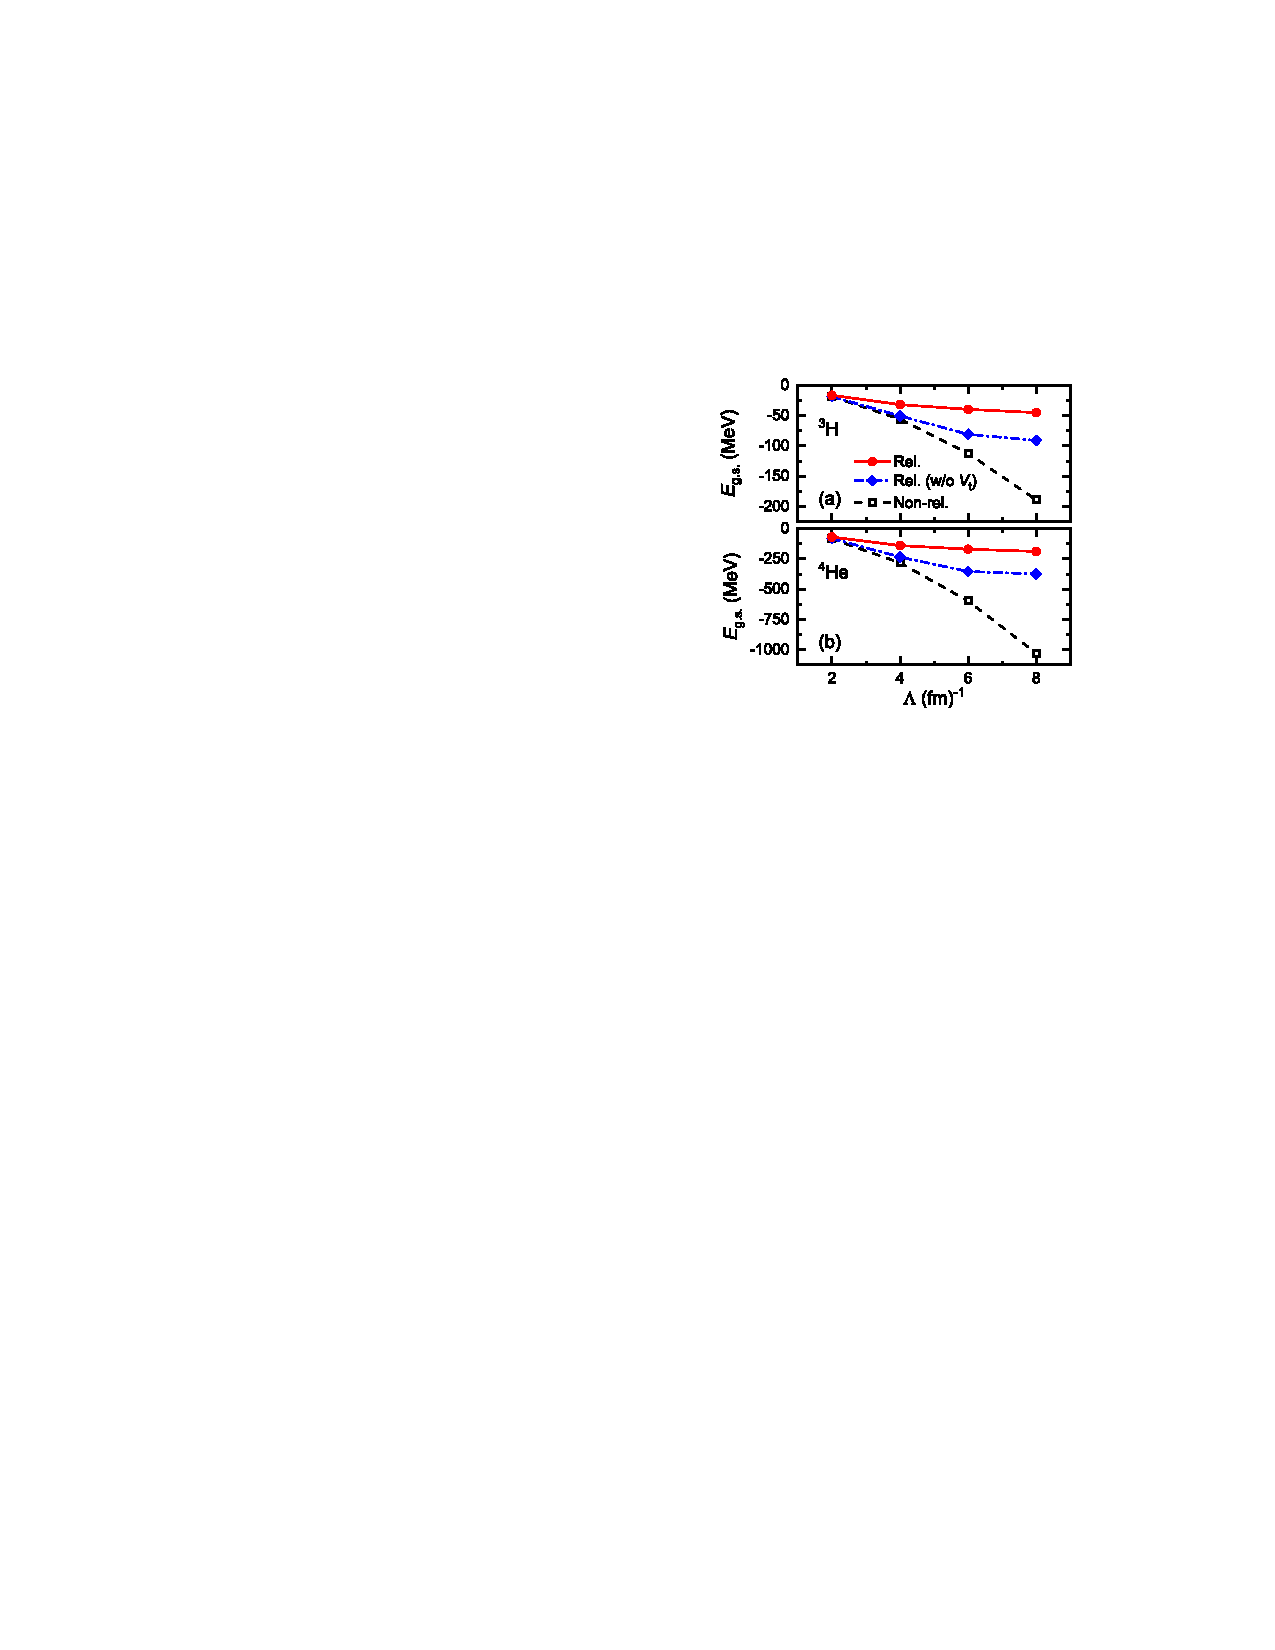
\includegraphics[width=0.55\linewidth]{figures/applications/relativistic.pdf}
\caption{\label{fig:relativistic_nuclei} 
(From Ref.~\cite{yang_consistent_2022} with permission from the Authors)
Ground-state energies of $^3$H (panel a) and $^4$He (panel b) obtained
with the nonrelativistic LO Hamiltonian and the relativistic ones
without and with ``transfer'' interactions, as functions of the cutoff
$\Lambda$.}
\end{figure}

Reproducing the experimental binding energies nevertheless requires a
$3N$ interaction. In this relativistic framework, the interplay between
relativistic corrections and the $3N$ force leads to a significant
suppression of three-body contributions to the binding energy, largely
independent of the strength of the $3N$ interaction. These findings,
obtained using VMC calculations based on SJ wave functions, provide the
first unified and internally consistent treatment of relativistic
dynamics and many-body forces in light nuclei, and open new avenues for
improving \emph{ab initio} calculations through a more complete
understanding of relativistic effects.



\subsubsection
{Reaching $^{16}$O with systematically improvable ansätze}

As discussed above, the SJ ansatz is not universal, since the Jastrow factor cannot remove the nodes generated by the mean-field component of the wave function. To address this limitation, the authors of Ref.~\cite{lovato_hidden-nucleons_2022} generalized the hidden-fermion family of NQS introduced in Ref.~\cite{moreno_fermionic_2022} to encompass both continuous and discrete degrees of freedom—see Sec.~\ref{sec:nqs} for a detailed discussion of the HN architecture. Using this framework, they solved the nuclear many-body Schr\"odinger equation in a systematically improvable manner. In particular, they showed that augmenting the original Hilbert space with HNs substantially enhances the expressivity of the neural-network ansatz compared to the SJ wave function.

The work in Ref.~\cite{lovato_hidden-nucleons_2022} also demonstrated that explicitly encoding parity and time-reversal symmetries in the wave function, as in Eqs.~\eqref{eq:psi_P} and~\eqref{eq:psi_PT}, significantly accelerates the training. In addition, the convergence of the SR algorithm is substantially improved by introducing the RMSProp-inspired regularization of Eq.~\eqref{eq:sr_rmsprop}. Figure~\ref{fig:sr_rmsprop}, taken from Ref.~\cite{lovato_hidden-nucleons_2022}, shows the convergence of the ground-state energy of $^3$H obtained with $A_h=3$ HNs and the positive-parity ansatz of Eq.~\eqref{eq:psi_P}. The orange solid circles, corresponding to energies obtained using the RMSProp-regularized SR scheme, are systematically closer to the numerically exact hyperspherical-harmonics result of Ref.~\cite{gnech_calculation_2020} than those obtained with the original SR algorithm, shown by solid blue circles. Moreover, the reduced scatter of the SR–RMSProp estimates compared to the SR results indicates improved stability of the optimization. Most notably, regardless of the specific regularization employed, both SR and SR–RMSProp yield energies that are appreciably lower than the SJ value reported in Ref.~\cite{Gnech2021}.

\begin{figure}[t]
\begin{center}
	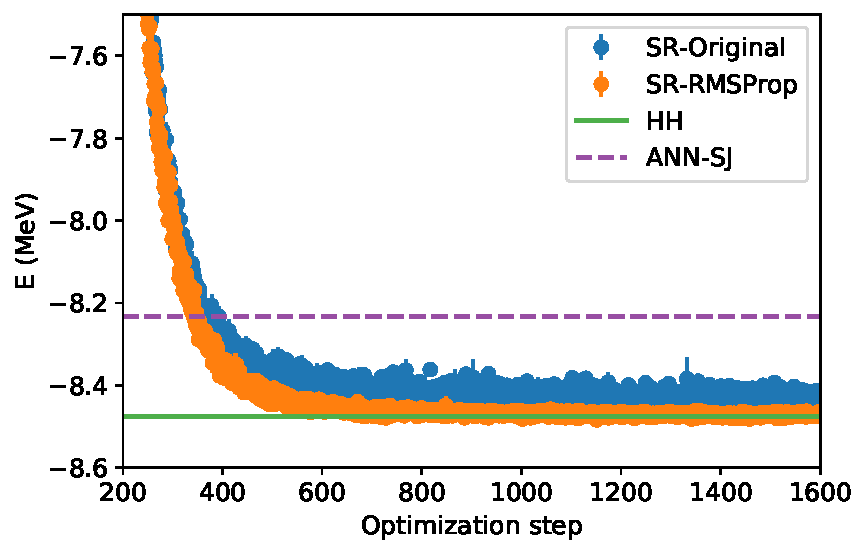
\includegraphics[width=0.6\textwidth]{figures/applications/h3_energies.pdf} 
	\caption{Convergence of the SR algorithm for $^3$H with the original (blue solid circles) and RMSProp-like (orange solid circles) diagonal shifts. The SJ and the HH energies of Ref.~\cite{Gnech2021} are displayed by the purple dashed and solid green lines, respectively.}
	\label{fig:sr_rmsprop}
\end{center}
\end{figure}

Reference~\cite{lovato_hidden-nucleons_2022} significantly extended the applicability of variational Monte Carlo calculations based on neural-network quantum states to nuclei as large as $^{16}$O, whereas earlier applications~\cite{adams_variational_2021,Gnech2021} were limited to systems with $A\leq 6$. The ground-state energy of $^{16}$O obtained with the HN ansatz was compared with results from the AFDMC method. In particular, comparisons were carried out both with variational energies obtained using the linearized ansatz of Eq.~\eqref{eq:variational_linear} and with full diffusion Monte Carlo results that include imaginary-time projection.

Figure~\ref{fig:16O_energy} displays the ground-state energy of $^{16}$O as a function of the number of HNs $A_h$ for the parity- and time-reversal-conserving ansatz of Eq.~\eqref{eq:psi_PT}. For reference, the VMC energy obtained with the correlation operator of Eq.~\eqref{eq:variational_linear} is indicated by the dashed green line, with the shaded band representing the corresponding Monte Carlo statistical uncertainty. The solid horizontal line and the associated shaded region denote the constrained-path AFDMC energy and its statistical uncertainty reported in Ref.~\cite{schiavilla_two-_2021}. Already for $A_h=2$, the HN wave function reproduces the VMC result. Upon further increasing $A_h$, the variational energy is progressively lowered and becomes consistent with the AFDMC value within uncertainties, demonstrating the accuracy of the HN ansatz for $p$-shell nuclei.



\begin{figure}[!htb]
\centering
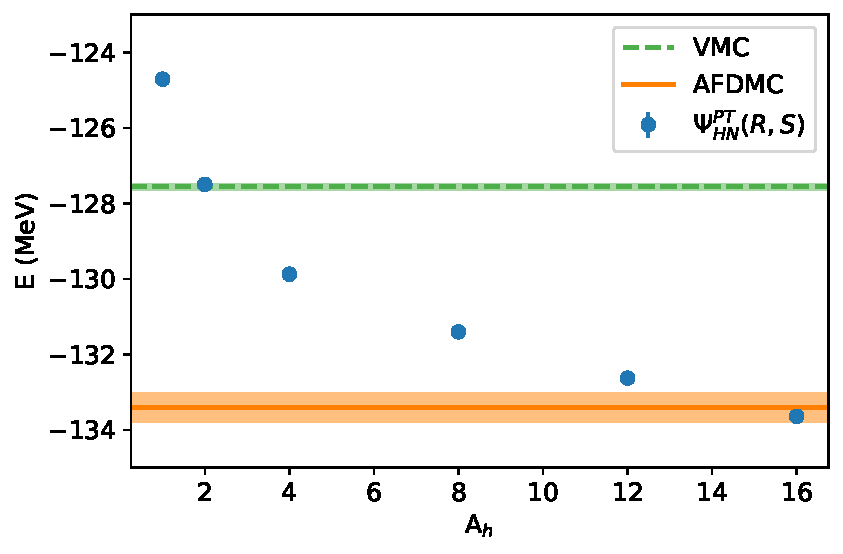
\includegraphics[width=0.6\textwidth]{figures/applications/o16_energies.pdf} 
\caption{Ground-state energy of $^{16}$O as a function of the number of hidden nucleons $A_h$ (solid blue points). The VMC and AFDMC energies—the latter taken from Ref.~\cite{schiavilla_two-_2021}—are shown by the dashed green and solid orange lines, respectively. The shaded areas represent the corresponding Monte Carlo statistical uncertainties.}
\label{fig:16O_energy}
\end{figure}

A comparable level of accuracy has been achieved in Ref.~\cite{Yang:2023rlw} by augmenting the SJ ansatz with a backflow transformation referred to as \emph{FeynmanNet}. In that work, the authors show that FeynmanNet yields very accurate ground-state energies and wave functions for $^4$He and $^6$Li, and extends to systems as large as $^{16}$O, using leading-order and next-to-leading-order Hamiltonians of pionless effective field theory. Notably, the latter include tensor components, which render the ground-state wave functions complex valued. More specifically, FeynmanNet uses a linear combination of Slater determinants together with a backflow transformation constructed from expressive deep neural networks that act on both the continuous spatial coordinates and the discrete spin–isospin degrees of freedom of the nucleons. To capture many-body correlations induced by tensor and spin–orbit interactions, the networks are designed to represent complex-valued nuclear wave functions. In addition, key features of low-energy nuclear structure, such as the major shell structure and relevant point symmetries, are explicitly encoded in the architecture. As a result, the FeynmanNet ansatz achieves high accuracy while remaining robust and efficient during the training process.

Figure~\ref{fig:feynmannet} illustrates the performance of the FeynmanNet architecture for $^4$He, $^6$Li, and $^{16}$O, using a linear combination of $N_{\rm det}=4$ Slater determinants. Panels (a)–(c) correspond to calculations performed with the model ``o'' Hamiltonian, also used in the HN calculations discussed earlier, which is based on a leading-order pionless effective field theory expansion. Panel (a) shows that the $^4$He energy rapidly converges to a ground-state value consistent with the numerically exact HH result, while improving upon the SJ ansatz. As emphasized in Ref.~\cite{Yang:2023rlw}, this improvement originates from the combined use of multiple determinants and a backflow transformation, which enhances the nodal structure in both spatial and spin–isospin degrees of freedom. For the $p$-shell nucleus $^6$Li, shown in panel (b), where clustering effects increase the complexity of the wave function, FeynmanNet yields lower variational energies than both the SJ ansatz and HH calculations, the latter exhibiting slow convergence for such a halo-like system~\cite{gnech_calculation_2020}. The expressive power of the approach is further demonstrated for $^{16}$O in panel (c), where FeynmanNet attains energies competitive with constrained-path AFDMC results within a purely variational framework. Notably, a comparison with Fig.~\ref{fig:16O_energy} indicates that FeynmanNet achieves lower variational energies than the HN ansatz.
Finally, panel (d) shows results for $^4$He obtained with a next-to-leading-order pionless effective field theory Hamiltonian from Ref.~\cite{schiavilla_two-_2021}, with a three-body range of $R_3 = 2.0$~fm. This Hamiltonian includes tensor and spin–orbit interactions that render the wave function complex valued and reduce the underlying symmetries. Despite this increased complexity, FeynmanNet retains a convergence rate comparable to the leading-order case and reaches energies consistent with HH calculations, highlighting the robustness of the ansatz.

\begin{figure}[!htb]
\centering
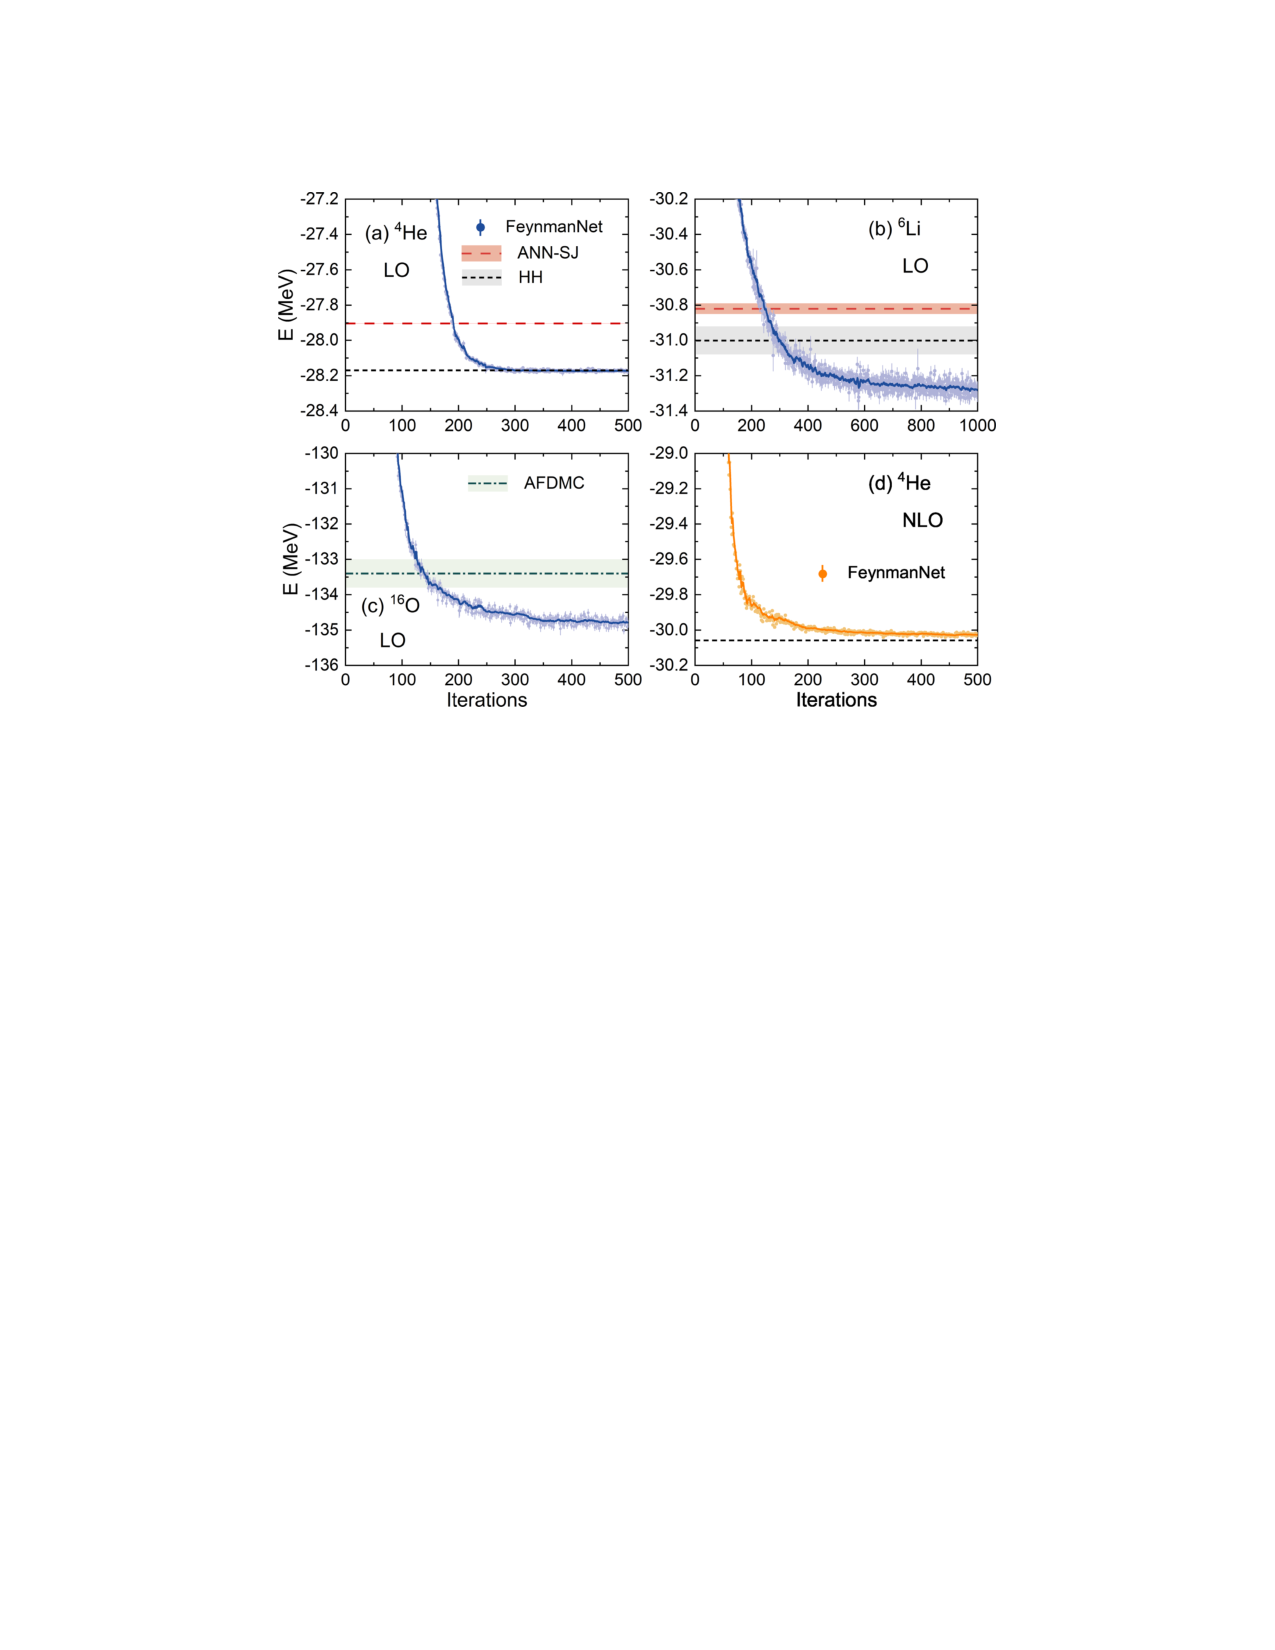
\includegraphics[width=0.8\textwidth]{figures/applications/feynmannet.pdf} 
\caption{Performance of the FeynmanNet ansatz for the ground states of $^4$He, $^6$Li, and $^{16}$O~\cite{Yang:2023rlw}. Panels (a)–(c) show the convergence of the ground-state energies obtained with the model ``o'' Hamiltonian. Statistical uncertainties from Monte Carlo sampling are indicated by error bars, while the solid curves represent exponential moving averages. Results obtained with the SJ ansatz and the HH method are shown for comparison where available. Panel (d) displays $^4$He results obtained with next-to-leading-order Hamiltonians. }
\label{fig:feynmannet}
\end{figure}


\subsubsection{Essential elements of nuclear binding}
The authors of Ref.~\cite{gnech_distilling_2024} improved the expressivity of the HN ansatz by introducing backflow transformations acting on the visible coordinates. In particular, they employed the equivariant backflow transformation defined in Eq.~\eqref{eq:mpnn}. The inclusion of backflow substantially increases the flexibility of the HN ansatz, allowing converged energies to be obtained with a HN number $A_h$ that is much smaller than the number of physical nucleons, and in some cases as small as a single HN. Figure~\ref{fig:hidden_backflow}, adapted from the Supplemental Material of Ref.~\cite{gnech_distilling_2024}, shows the convergence of the ground-state energy of $^{16}$O computed using Hamiltonian ``o'' of Ref.~\cite{schiavilla_two-_2021} with $R_3=1.0$, as a function of $A_h$. Even with $A_h=1$, the resulting energy is lower than that obtained with $A_h=16$ in the absence of a backflow transformation. The converged energy is consistent, within uncertainties, with that obtained using the FeynmanNet ansatz, shown in Fig.~\ref{fig:feynmannet}, as well as with the constrained-path AFDMC value.

\begin{figure}[!htb]
\centering
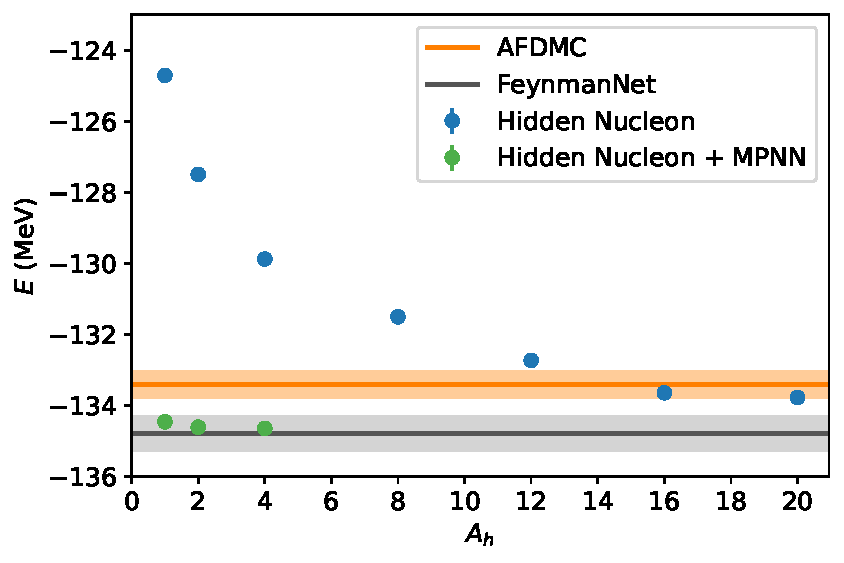
\includegraphics[width=0.6\textwidth]{figures/applications/hidden_backflow.pdf} 
\caption{Adapted from Ref.~\cite{gnech_distilling_2024} with permission from the authors. Ground-state energy of $^{16}$O obtained using the Hamiltonian “o” of Ref.~\cite{schiavilla_two-_2021} with $R_3=1.0$ fm. The HN results of Ref.~\cite{lovato_hidden-nucleons_2022} are compared with those obtained by incorporating the simple message-passing neural networks backflow transformations introduced in Ref.~\cite{gnech_distilling_2024}. For reference, the auxiliary-field diffusion Monte Carlo (AFDMC) energy from Ref.~\cite{schiavilla_two-_2021}, together with its uncertainty, is shown by the orange shaded band, while the best FeynmanNet energy reported in Ref.~\cite{Yang:2023rlw} is indicated by the gray band.}
\label{fig:hidden_backflow}
\end{figure}

This architecture, employing up to $A_h = 4$ HN to ensure convergence, has been used to compute the ground-state energies per nucleon of selected nuclei with $A \leq 20$ for $R_3 = 1.0$ fm and $R_3 = 1.1$ fm. As shown in the top panel of Fig.~\ref{fig:spectrum_radii}, the agreement between the computed and experimental values is remarkably good, given the simplicity of the input Hamiltonian. As noted by the authors of Ref.~\cite{gnech_distilling_2024}, the ground-state energies obtained with this simple Hamiltonian are closer to experiment than those reported in Ref.~\cite{martin_auxiliary_2023} using AFDMC with N$^2$LO chiral EFT interactions. In addition, unlike in NCSM calculations employing consistent N$^2$LO NN and 3N forces~\cite{maris_light_2021}, no increasing overbinding with mass number $A$ is observed.
An important caveat, however, is that neither $R_3 = 1.0$ fm nor $R_3 = 1.1$ fm yield bound ground states for $^6$He, $^8$Li, $^8$B, $^9$C, and $^{17}$F with respect to breakup into smaller clusters. This behavior points to an excessively repulsive character of the Hamiltonian, since increasing $A_h$, and thus the flexibility of the NQS, does not lead to an improvement of the variational energies.

The corresponding charge radii are shown in the lower panel of Fig.~\ref{fig:spectrum_radii}. While the overall trend of the experimental data is well reproduced, consistent with the ground-state energies, the radii of $^6$Li, $^7$Li, $^7$Be, and $^{12}$C are overestimated. By contrast, the radii of $^{15}$N, $^{16}$O, $^{17}$O, and $^{20}$Ne are underestimated with respect to experiment, particularly for $R_3 = 1.0$ fm. Owing to its longer range, the 3N interaction with $R_3 = 1.1$ fm introduces additional repulsion and leads to larger radii in nuclei with $A \geq 15$ compared to the interaction with $R_3 = 1.0$ fm. In contrast to methods based on harmonic-oscillator basis expansions~\cite{caprio_robust_2022}, the radii converge rapidly in VMC-NQS calculations. Consequently, the discrepancies between theoretical predictions and experimental data are most likely attributable to deficiencies in the input Hamiltonian. 

\begin{figure}[!htb]
\centering
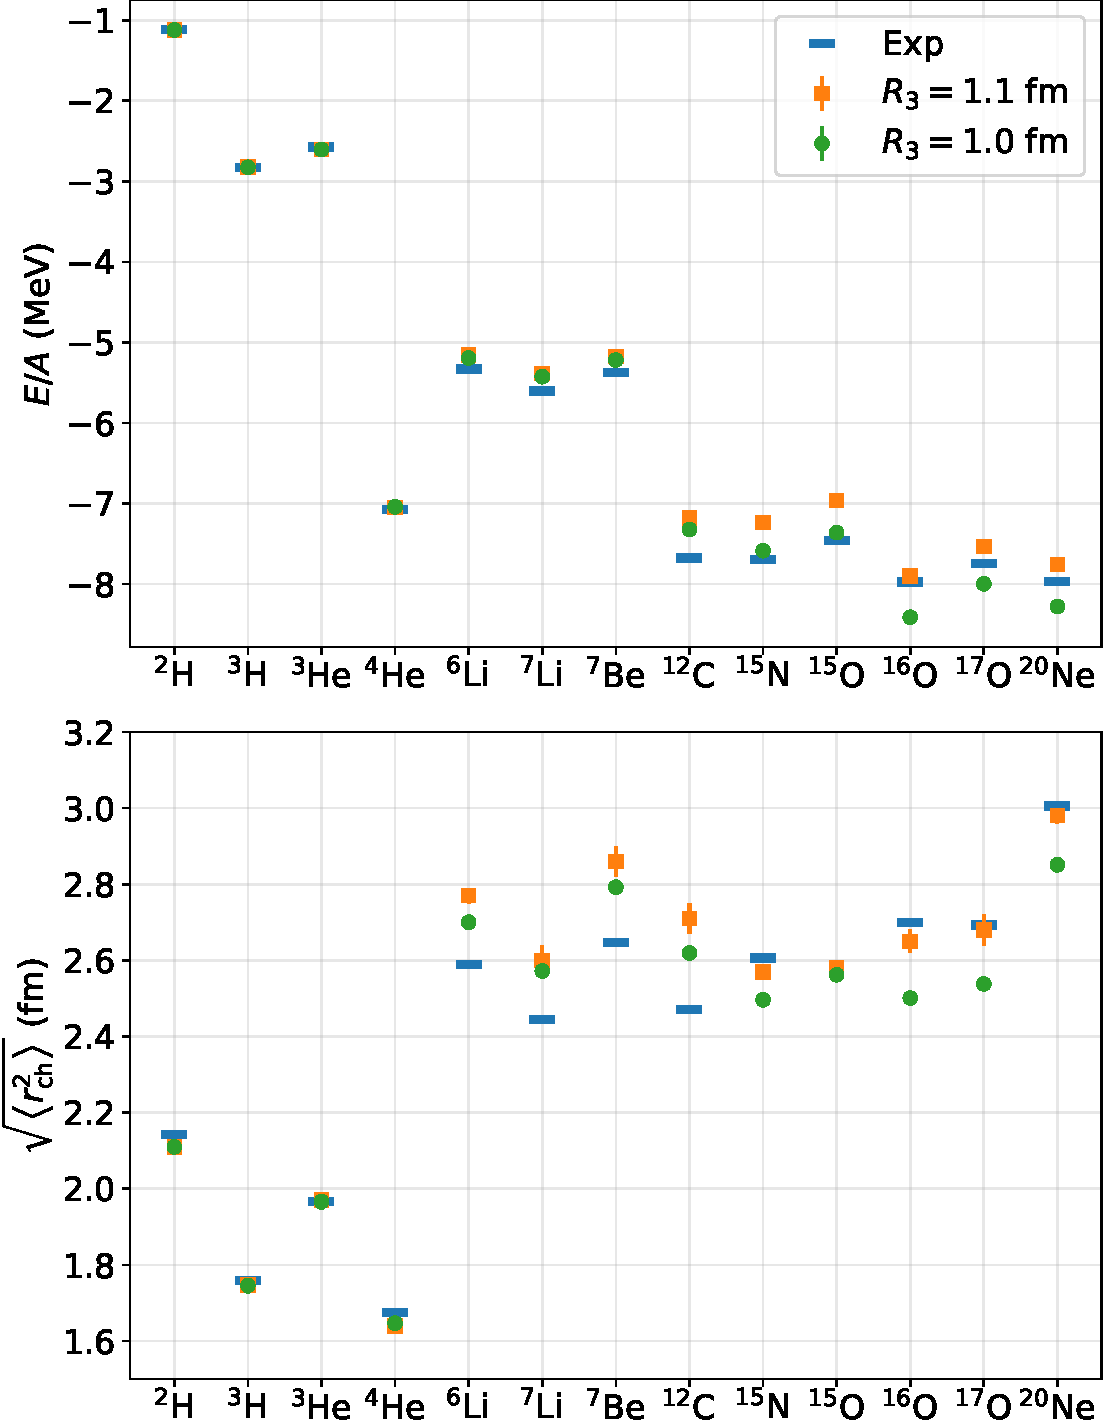
\includegraphics[width=0.55\textwidth]{figures/applications/spectrum_radii.pdf} 
\caption{Adapted from Ref.~\cite{gnech_distilling_2024} with permission from the authors. Energies per particle (upper panel) and charge radii (lower panel) of selected nuclei with up to $A = 20$ obtained using the Hamiltonian “o” of Ref.~\cite{schiavilla_two-_2021} with $R_3 = 1.0$ fm and $R_3 = 1.1$ fm, compared with experimental data. }
\label{fig:spectrum_radii}
\end{figure}

The magnetic moments of selected nuclei with $A \leq 20$, computed using model “o” with $R_3 = 1.1$ fm, are shown in Fig.~\ref{fig:moments}. The theoretical predictions are in good agreement with experimental data, indicating that the NQS captures the nuclear shell structure, which emerges naturally during the energy minimization. Notably, at the beginning of the training, not only the ground-state energies and charge radii, but also the magnetic moments and angular momenta, differ substantially from their converged and experimentally observed values. The minor discrepancies observed for $^3$H and $^3$He, consistent with GFMC, AFDMC, and HH results~\cite{pastore_quantum_2013,gnech_magnetic_2022,martin_auxiliary_2023}, are likely due to missing two-body current contributions.

\begin{figure}[!htb]
\centering
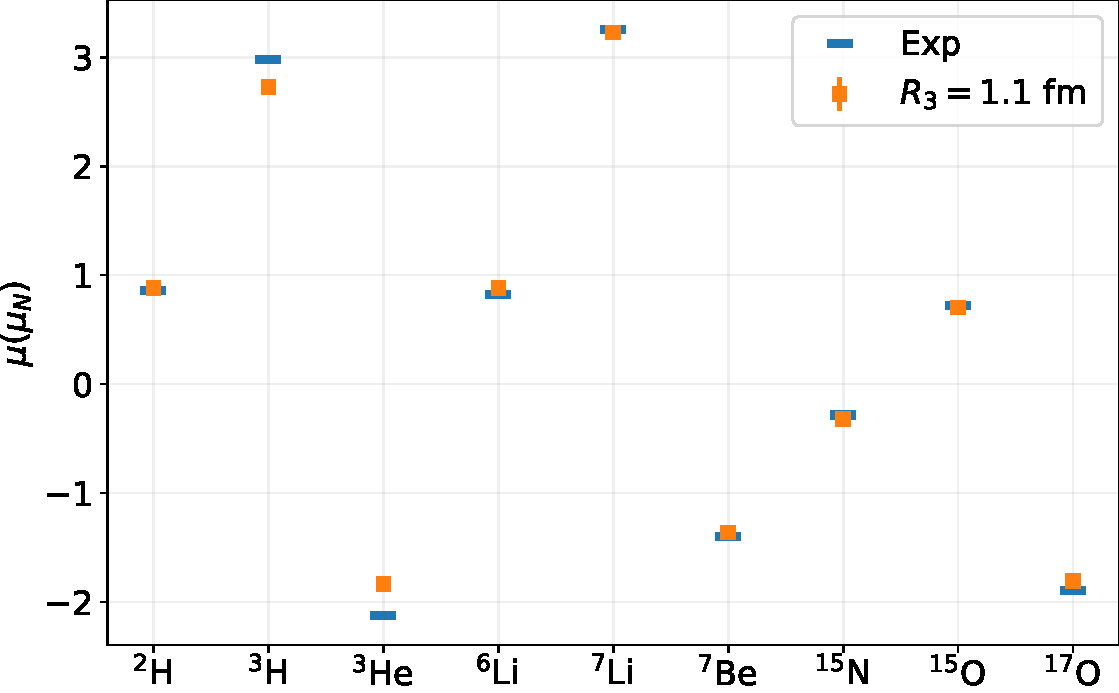
\includegraphics[width=0.55\textwidth]{figures/applications/magnetic_moments.pdf} 
\caption{Adapted from Ref.~\cite{gnech_distilling_2024} with permission from the authors. Magnetic moments of selected nuclei with $A \leq 20$ obtained from VMC-NQS calculations using the Hamiltonian “o” of Ref.~\cite{schiavilla_two-_2021} with $R_3 = 1.1$ fm, compared with experimental data.}
\label{fig:moments}
\end{figure}

\subsubsection[High-resolution potentials]{High-resolution potentials}

Most nuclear-physics applications of VMC methods with NQS take as input interactions based on pionless effective field theory. After the pioneering 2019 work~\cite{keeble_machine_2020}, non-stochastic NQS-based approaches have been employed to solve light nuclear systems with high-resolution interactions. In this context, the authors of Ref.~\cite{wang_neural_2024} introduced a compact neural-network architecture based on a partial-wave expansion of the nuclear wave function, in which the radial components are represented by separate neural networks. This method was shown to accurately reproduce the deuteron ground-state energy and wave function starting from the highly realistic Argonne $v_{18}$ NN potential~\cite{wiringa_accurate_1995}, including its full spin–isospin operator structure. More recently, closely related deterministic neural-network approaches have been extended beyond the two-body sector. In particular, Ref.~\cite{li_solving_2025} introduced an unsupervised deep-learning framework to solve both two- and three-body bound-state problems directly in coordinate space. Building on a discretized representation of the Schrödinger equation, the authors employed deep neural networks to represent the radial wave functions of coupled channels, achieving accurate calculations of $^2$H and $^3$H using the Entem–Machleidt N$^3$LO chiral-EFT potential of Ref.~\cite{Entem2003}.

By contrast, actual VMC calculations based on NQS have more recently been carried out using high-resolution local Hamiltonians that are either phenomenological or derived within chiral EFT~\cite{yang_chiral_2025,wen_neural-network_2025,yang_zemach_2025}. In particular, the authors of Ref.~\cite{yang_chiral_2025} presented QMC calculations of neutron–$\alpha$ D-wave phase shifts using chiral-EFT Hamiltonians at the three lowest orders in the chiral expansion: LO, NLO, and N$^2$LO. Specifically, they employed the local $NN$ and $3N$ potentials constructed in Ref.~\cite{gezerlis_quantum_2013,lynn_quantum_2014}. However, the analysis was limited to the softest cutoff value, $R_0 = 1.2$ fm, which corresponds to a typical momentum cutoff $\Lambda \simeq 400$ MeV.

As in previous QMC studies of neutron--$\alpha$ scattering, the continuum problem is mapped onto a bound-state eigenvalue problem. To this end, an external harmonic-oscillator (HO) confining potential is added to the nuclear Hamiltonian through an additional two-body term of the form
\begin{equation}
V_{\text{HO}} = \sum_{i<j} \frac{1}{2}\,\frac{m_N}{A}\,\omega^2 r_{ij}^2 \, ,
\end{equation}
where $m_N$ denotes the nucleon mass, $\omega$ the HO frequency, and $r_{ij}$ the relative distance between nucleons. The presence of the HO trap discretizes the spectrum, enabling the extraction of scattering information from bound-state energies. The neutron--$\alpha$ D-wave phase shifts are then obtained using the Busch--Englert--Rza\.{z}ewski--Wilkens (BERW) formalism~\cite{busch_two_1998,buttiker_pionnucleon_2000}, which relates the trapped eigenenergies of $^5$He and the ground-state energy of $^4$He to free-space scattering observables.

In Ref.~\cite{yang_chiral_2025}, the energies of both $^4$He and $^5$He are computed using the GFMC method. The lowest $J^\pi = 5/2^+$ eigenstate of $^5$He is projected via imaginary-time propagation, starting from a previously optimized NQS. The trial wave function is taken in the form of Eq.~\eqref{eq:SJ_chiral}, augmented by the transformation defined in Eq.~\eqref{eq:SJ_chiral_2}.
Despite the use of highly sophisticated variational wave functions, the GFMC propagation suffers from a severe fermion-sign problem. This issue is mitigated through a combination of constrained-path propagation followed by a transient estimate~\cite{wiringa_quantum_2000}. Nevertheless, the sign problem remains sufficiently severe that only the softest available cutoff value, $R_0 = 1.2$ fm, could be employed in the chiral nuclear Hamiltonian.

\begin{figure}[!htb]
\centering
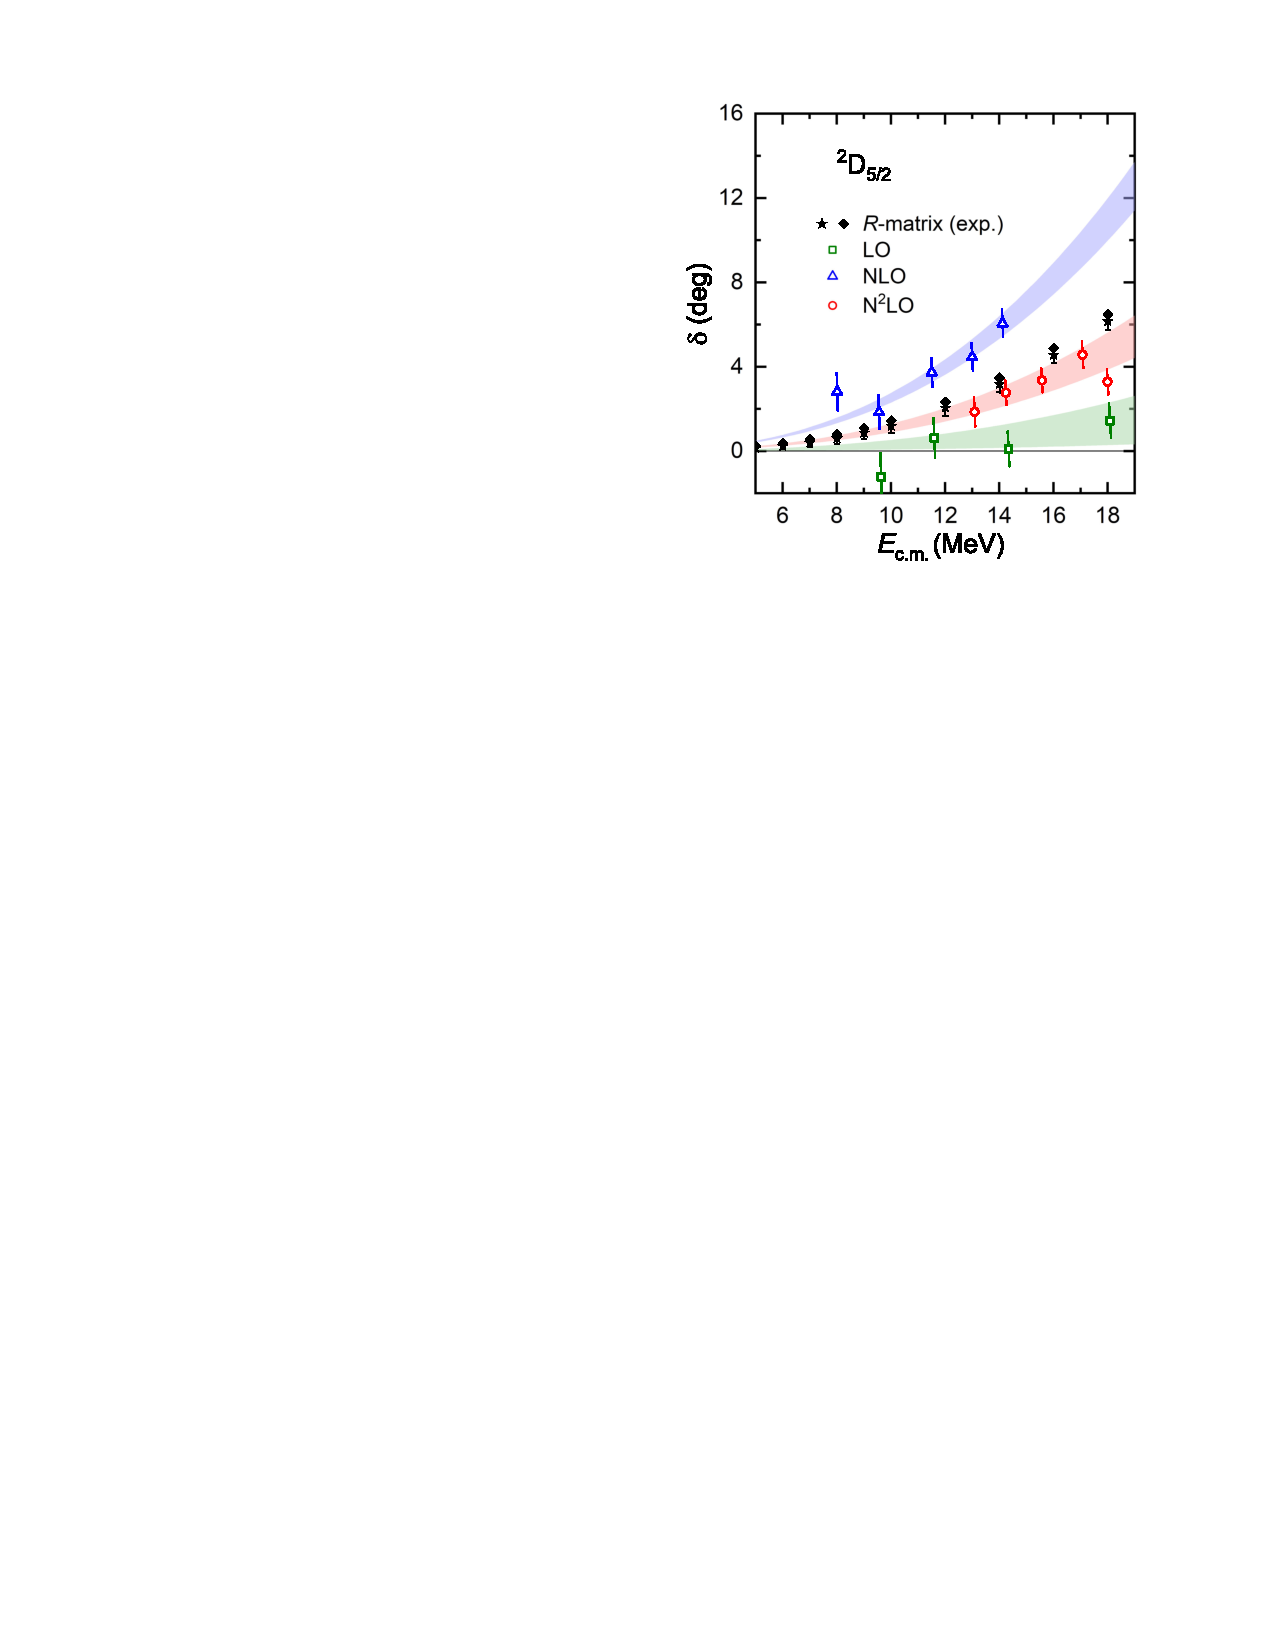
\includegraphics[width=0.5\columnwidth]{figures/applications/n_alpha_scattering.pdf}
\caption{From Ref.~\cite{yang_chiral_2025}, reproduced with permission. Neutron–$\alpha$ phase shifts in the ${}^2D_{5/2}$ channel as a function of the center-of-mass energy, predicted at different orders of chiral EFT. Empty symbols denote GFMC results with statistical error bars, while shaded bands indicate the combined statistical and BERW-related systematic uncertainties. Stars correspond to $R$-matrix analyses of experimental neutron–$\alpha$ elastic-scattering data~\cite{bond_determination_1977}, and red diamonds are taken from a private communication between the authors of Ref.~\cite{yang_chiral_2025} and G.~M.~Hale.}
\label{fig:n_alpha_scattering}
\end{figure}

Figure~\ref{fig:n_alpha_scattering} illustrates the neutron–$\alpha$ D-wave phase shifts predicted at different orders of chiral EFT as a function of the center-of-mass energy $E_{\rm c.m.}$. Each point corresponds to an individual GFMC calculation performed in a harmonic-oscillator trap and is extracted using the BERW formalism. The theoretical predictions are compared with phase shifts obtained from $R$-matrix analyses of elastic-scattering data~\cite{bond_determination_1977}.
At leading order, the chiral Hamiltonian yields nearly vanishing phase shifts, in line with general expectations. The dominant contribution emerges at next-to-leading order with the inclusion of the two-pion-exchange $NN$ interaction, but the resulting phase shifts significantly overestimate the empirical values. Corrections at next-to-next-to-leading order reduce the phase shifts and bring the theoretical predictions into closer agreement with the data. At this order, the leading $3N$ force plays a crucial role, while the subleading two-pion-exchange $NN$ interaction has a comparatively minor impact for the soft regulator values considered. Overall, these results identify neutron–$\alpha$ D-wave scattering as a sensitive probe of the long-range structure of the three-nucleon interaction.

In a later work~\cite{yang_zemach_2025}, the same authors improved their variational ansatz by adopting a fully multiplicative form of two-body correlations, rather than the linearized version of Eq.~\eqref{eq:SJ_chiral}. Using this more sophisticated wave function, they computed the binding energies of $^4$He and $^6$Li with accuracy comparable to GFMC and significantly improved relative to earlier VMC and AFDMC calculations. Notably, because VMC does not suffer from a fermion-sign problem, they were able to employ local chiral-EFT interactions from Refs.~\cite{gezerlis_quantum_2013,lynn_quantum_2014} with both $R_0 = 1.2$ fm and the harder cutoff $R_0 = 1.0$ fm. In addition, they considered the high-resolution phenomenological Argonne $v_8^\prime$ plus UIX Hamiltonian.

These calculations resolved the longstanding discrepancy between effective and elastic Zemach radii in $^6$Li and $^7$Li through ab initio nuclear-structure calculations that consistently include nuclear polarizability effects. Enabled by the use of highly sophisticated NQS, the results show that nuclear polarizability effects are negligible in $^7$Li but dominant in $^6$Li, thereby accounting for the observed deviation between the effective and elastic Zemach radii.

The authors of Ref.~\cite{wen_neural-network_2025} employed the wave-function ansatz of Eq.~\eqref{eq:wen_u_corr} to study $A = 3$ nuclei, using as input the local chiral-EFT Hamiltonians of Refs.~\cite{gezerlis_local_2014,lynn_chiral_2016}. Importantly, these interactions include tensor and spin–orbit components in the $NN$ sector, as well as a consistent spin-isospin-dependent three-nucleon force. As discussed in Section~\ref{sec:chiral_ansatz}, a normalizing flow is used to generate the samples required for the Monte Carlo estimation of the energy and its gradient. Notably, the use of normalizing flows avoids the correlation-length problem that typically affects Markov chain Monte Carlo algorithms.

\begin{figure}[!htb]
\centering
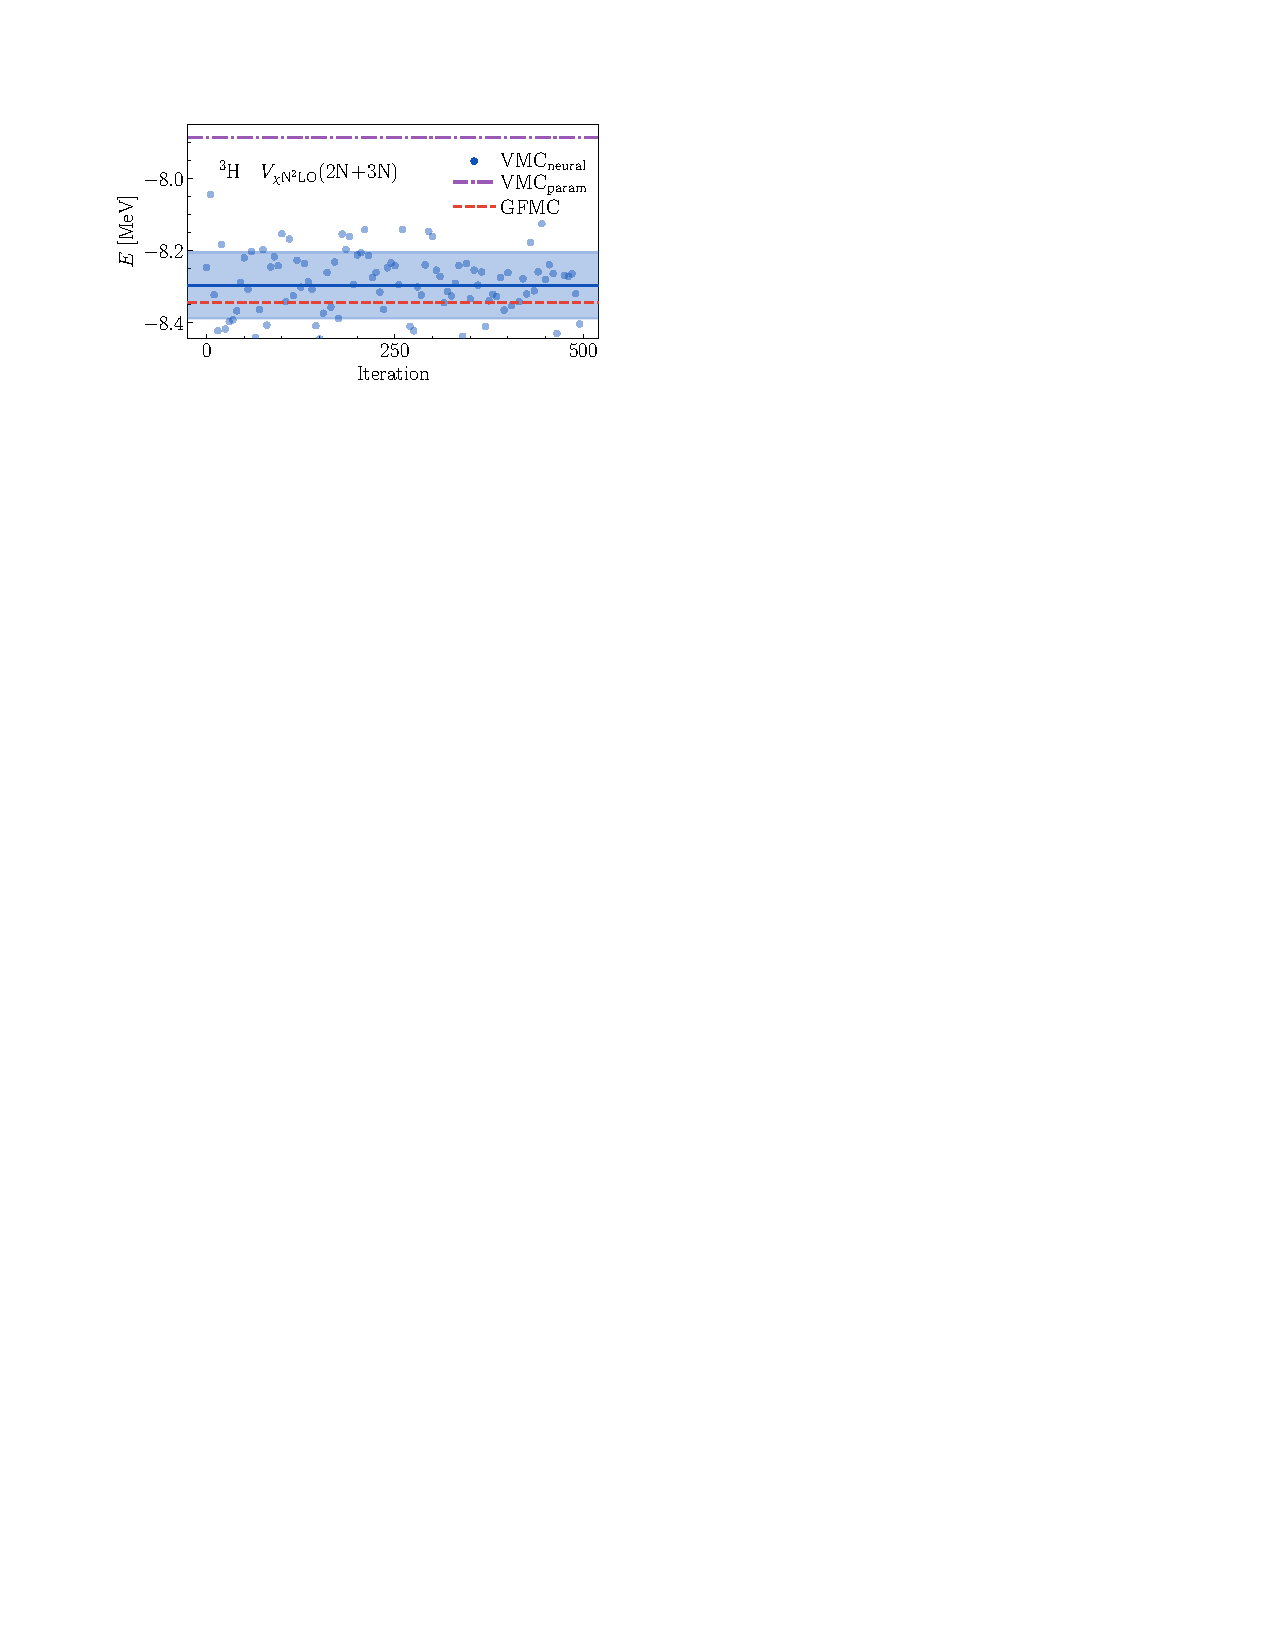
\includegraphics[width=0.6\columnwidth]{figures/applications/chiral_A_3.pdf}
\caption{From Ref.~\cite{wen_neural-network_2025}, reproduced with permission. Evaluation of the $^3$H ground-state energy obtained with optimized neural-network wave functions using the full N$^2$LO chiral interaction with $(R_0,\Lambda) = (1.2\,\mathrm{fm}, 1\,\mathrm{GeV})$. The average energy (blue horizontal line) and standard deviation (blue shaded band) are estimated over 500 iterations with 40{,}000 samples per iteration. The conventional VMC result is displayed by the purple line}
\label{fig:chiral_A_3}
\end{figure}

Figure~\ref{fig:chiral_A_3} displays the ground-state energy of $^3$H obtained using the N$^2$LO chiral interaction with regulator values $(R_0,\Lambda) = (1.2,\mathrm{fm}, 1,\mathrm{GeV})$. The energy and its uncertainty are estimated over 500 iterations, with 40,000 samples per iteration generated by the normalizing flow. The average NQS energy is $E = -8.30 \pm 0.09$ MeV, which closely matches the GFMC result, $E = -8.34$ MeV. The two values agree within one-half of a standard deviation and differ by only $0.45$\%.

These results indicate that the neural-network-generated wave function can effectively approximate the $^3$H ground state with the soft-core interaction, without any imaginary-time evolution, even in the presence of complicated pion-exchange terms as well as tensor, spin-orbit, charge-independence-breaking, and charge-symmetry-breaking interactions.


\subsection{Nuclear matter}
\label{sub:matter}

Multi-messenger astronomy is creating new observations of matter at densities and isospin asymmetries which are not directly accessible by terrestrial experiments, expanded most recently with the observation of GW170817~\cite{LIGOScientific:2017vwq,Abbott:2017,Sabatucci:2020xwt,senger2021}. Theoretical modeling of this matter, in particular material similar to the inner crust of neutron stars, poses significant challenges due to the inherent complexity of clustering phenomena, the emergence of superfluidity, and the existence of both free neutrons and neutron-rich nuclei. Various phenomenological approaches have been developed to address some of these challenges, including the compressible liquid-drop model~\cite{ Baym:1971ax,Baym:1971pw,Ravenhall:1983uh,douchin2001,Newton:2011dw,Gulminelli:2015csa,Lim:2017luh,Carreau:2019zdy,Grams:2021lzx} and self-consistent mean-field models~\cite{negele1973a,Baldo:2006jr,Grill:2011dr}. In the former, the energy is parameterized as a function of global properties, and the nucleons within clusters are treated separately from the free neutrons, all of which are assumed to be uniformly distributed. While this treatment has a low computational cost, it neglects quantum mechanical shell effects, which are critical for determining the equilibrium composition of the crust. In contrast, self-consistent mean-field models are fully quantum mechanical, constructing the many-body state in terms of single-particle or quasi-particle wave functions. However, since they neglect correlations beyond the mean-field approximation, they have limited applicability for low-density nuclear matter, where strong correlations may lead to significant deviations from the mean-field behavior.

Recently, VMC methods utilizing NQS have been used to model nuclear matter without making similar, limiting assumptions within both pure neutron matter (PNM) and symmetric nuclear matter (SNM) using a pionless EFT potential~\cite{fore2023,fore_investigating_2024}. The initial results show promise through capturing signs of density dependent neutron superfluidity in PNM as well as successfully modeling clustering in nuclear matter, without any assumptions on the structure of the material.


\subsubsection{Pure neutron matter}

\begin{figure}[!htb]
\centering
    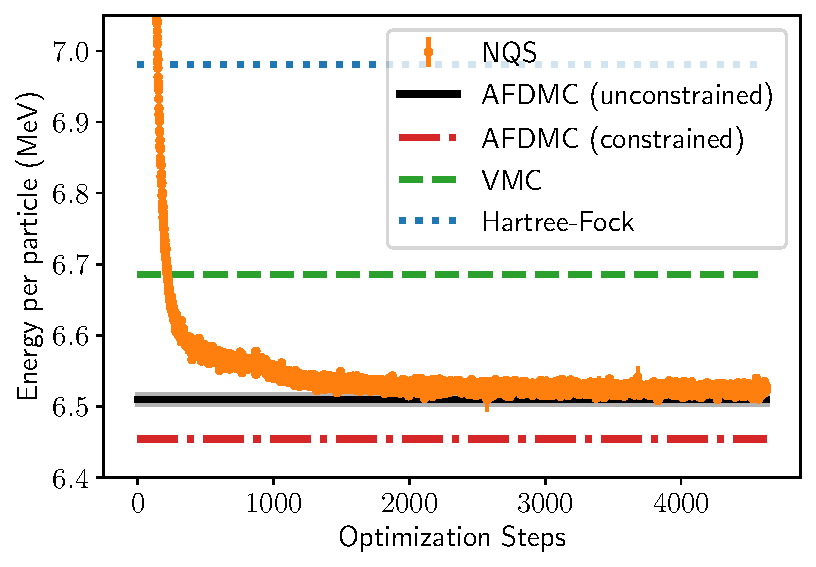
\includegraphics[width=0.6\columnwidth]{figures/nuclear_matter/PNM_04_training.pdf}
\caption{NQS training data in neutron matter at $\rho = 0.04$ fm$^{-3}$ (data points) compared with Hartree-Fock (dotted line), conventional VMC (dashed line), constrained-path AFDMC (dash-dotted line) and unconstrained-path AFDMC results (solid line).}
\label{fig:PNM_training}
\end{figure}

Low-density neutron matter is characterized by fascinating emergent quantum phenomena, such as the formation of Cooper pairs and the onset of superfluidity.
Quantum Monte Carlo approaches~\cite{carlson_quantum_2015}, in particular the auxiliary-field diffusion Monte Carlo (AFDMC) method~\cite{Schmidt:1999lik}, have been extensively applied to accurately compute neutron-matter properties~\cite{lonardoni_nuclear_2020,piarulli_benchmark_2020,Lovato:2022apd}. In the low-density regime, AFDMC calculations have convincingly shown a depletion of the superfluid gap with respect to BCS theory~\cite{Gandolfi:2008id,Gandolfi:2022dlx}. However, because of the fermion sign problem, AFDMC predictions depend upon the starting variational wave function. For instance, the superfluid phase must be assumed {\it a priori}. No assumption of the phase is necessary when NQS are used to compute the initial variational state. It can be seen in Fig.~\ref{fig:PNM_training} that the final trained state for a simulation of 14 neutrons with periodic boundary conditions that the variational NQS is able to recover almost an identical ground state energy to the unconstrained AFDMC calculation.

\begin{figure}
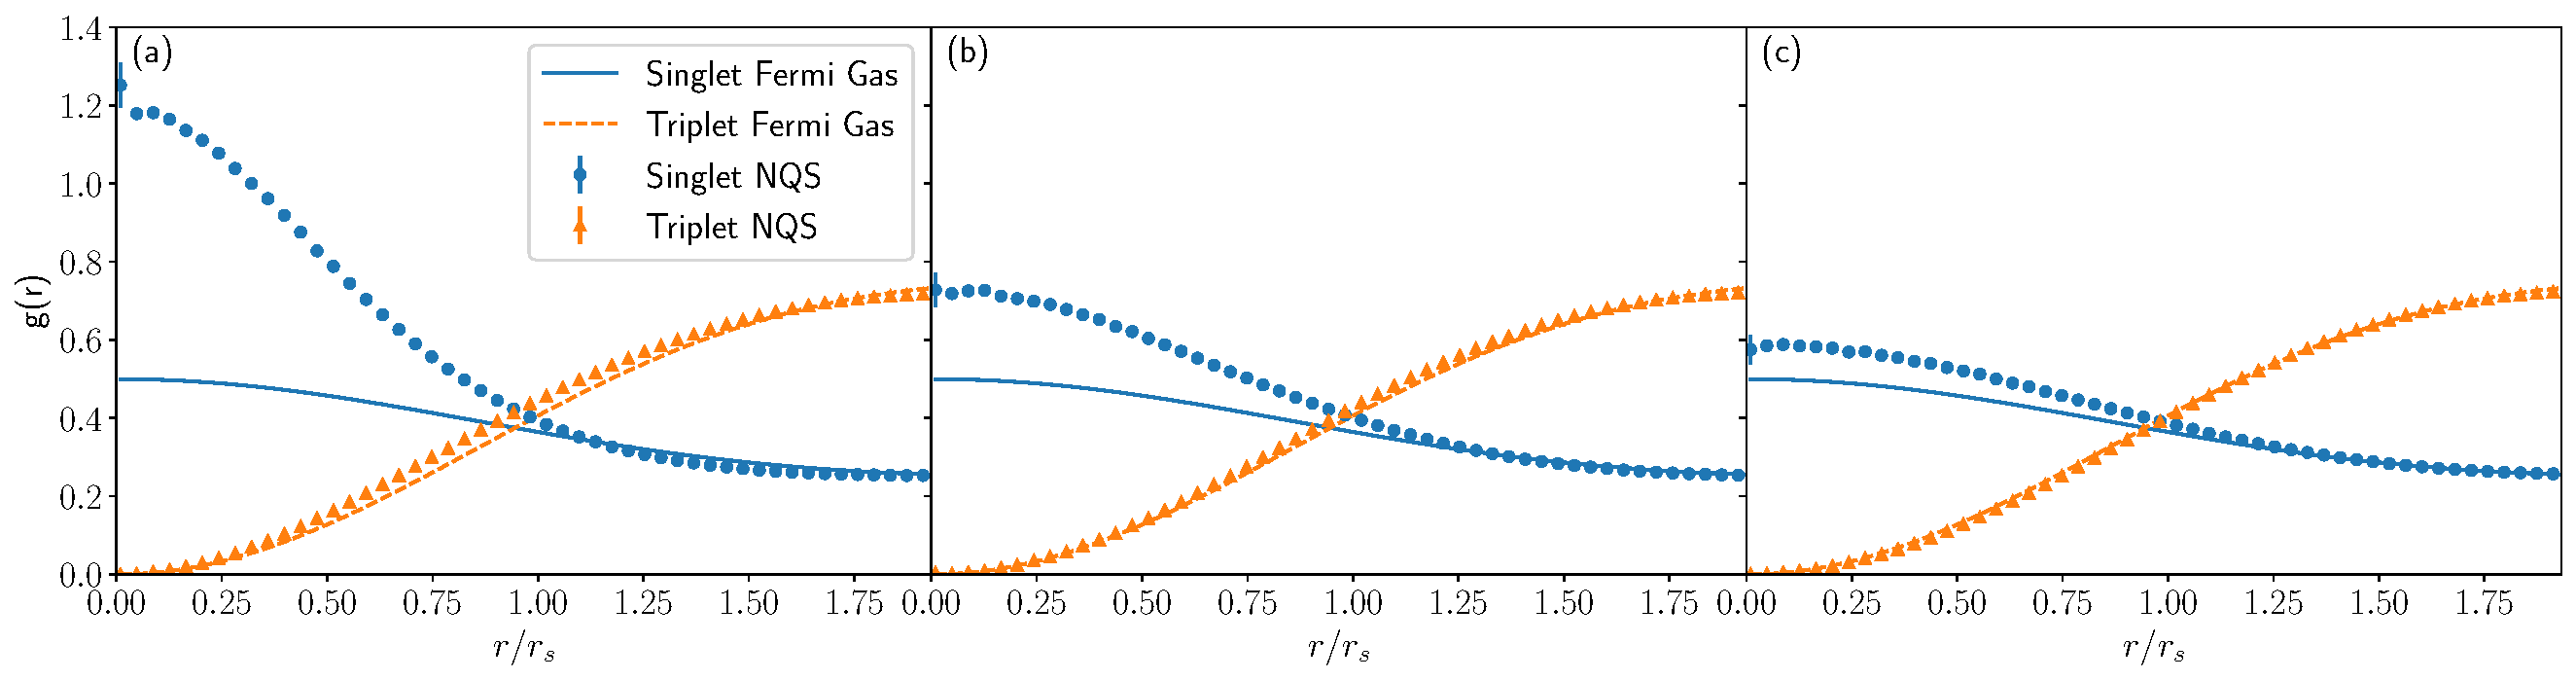
\includegraphics[width=\columnwidth]{figures/nuclear_matter/PNM_pair_dist_func_combined_wsr.pdf}
\caption{Spin-singlet and triplet two-body distribution functions at $\rho=0.01$ fm$^{-3}$ (panel a), $\rho = 0.04$ fm$^{-3}$ (panel b), and $\rho = 0.08$ fm$^{-3}$ (panel c) vs pair distance in units of the Wigner-Seitz radius. The NQS calculations (solid symbols) are compared with non-interacting Fermi Gas results (solid lines).}
\label{fig:pair_dist}
\end{figure}

The trained NQS wave functions from these simulations are also used to evaluate two-body pair distributions as defined in Ref.~\cite{Gandolfi2009}. Fig.~\ref{fig:pair_dist} shows these distributions at $\rho=0.01$ fm$^{-3}$ (panel a), $\rho=0.04$ fm$^{-3}$ (panel b), and $\rho=0.08$ fm$^{-3}$ (panel c). The significant increase in the spin-singlet channel compared to the non-interacting Fermi Gas indicates that the NQS wave function can capture the emergence of the $^1S_0$ neutron pairing, despite not being explicitly encoded in the ansatz. Consistent with the behavior of the pairing gap~\cite{Gandolfi:2008id,Benhar:2017mof}, the enhancement is more prominent at low densities and vanishes at higher densities. On the other hand, at these densities, no pairing correlations are present in the spin-triplet channel.

\subsubsection{Clustering}

Simulations of matter with protons as well as neutrons are complicated by the nuclear interaction acting simultaneously in distinct spin-isospin channels, most notably the $^1S_0$ and $^3S_1$ channels, rather than collapsing to a single dominant channel as in pure neutron matter (see Section \ref{sub:hamiltonian}). This richer structure leads to pronounced clustering that is difficult for many methods to capture without simplifying assumptions. NQS, however, excel at learning these complex relationships. 

Reference~\cite{fore_investigating_2024} utilizes the MPNN backflow method with the Pfaffian--Jastrow architecture to efficiently learn pairing correlations within isospin symmetric and asymmmetric matter. With this approach, NQS are able to correctly learn the structure of matter through a range of densities corresponding to the inner crust of neutron stars. Figure~\ref{fig:SNM_energy} shows ground state energies learned by the NQS are significantly improved compared to state-of-the-art AFDMC calculations given identical assumptions. For a simulation containing 28 particles, the expected low-density limit of periodic symmetric matter corresponds to the ground-state energy of $^{28}$Si in the absence of electromagnetic interactions. The NQS results approach this limit, providing clear evidence that clustering effects are being accurately captured. Further improvements may be achieved by initializing AFDMC calculations from a NQS wave function. 

\begin{figure}[!t]
\centering
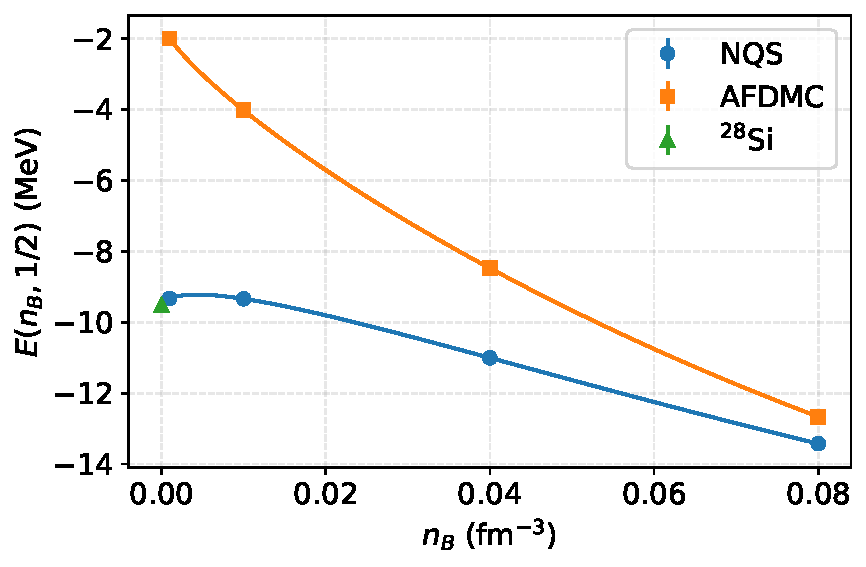
\includegraphics[width=0.6\columnwidth]{figures/nuclear_matter/SNM_energy.pdf}
\caption{Energy per particle of SNM from NQS and AFDMC simulations. The NQS results (blue circles) indicate stronger binding compared to AFDMC (orange squares), attributed to clustering at low densities. Our low-density results are compared to $^{28}$Si with no electromagnetic contribution, which serves as the expected zero-density ground state for a simulation of $N=28$ nucleons with $x=1/2$. The error bars represent 95\% confidence intervals for the mean.}
\label{fig:SNM_energy}
\end{figure}

%\begin{figure*}[!h]
%    \centering
%    \includegraphics[width=0.6\textwidth]{figures/nuclear_matter/SNM_config_25_25.pdf}

%    \caption{Example many-body configurations at different densities and proton fractions. Panels (a) and (b) correspond to proton fractions of $x=1/2$ and $x=4/28$, respectively, with a fixed baryon density of $n_B = 0.01$ fm$^{-3}$.
%    In these panels, the origin has been shifted to center the clusters of protons within each cell. Panels (c) and (d) correspond to proton fractions of $x=1/2$ and $x=4/28$, respectively, with a fixed baryon density of $n_B = 0.08$ fm$^{-3}$. A series of animations for \(x=4/28\) and \(x=1/2\) at \(0.01\), \(0.04\), and \(0.08\) fm\(^{-3}\), as well as for \(x=1/2\) at \(n_B=0.001\) fm\(^{-3}\), are publicly available at \href{https://github.com/kim-jane/Neutron_Star_Crust}{https://github.com/kim-jane/Neutron\_Star\_Crust}.}
%    \label{fig:SNM_3d_config}
%\end{figure*}


\subsubsection{Beta-equilibrated matter}

Cold nuclear matter at densities found in the inner crust of neutron stars is mostly composed of neutrons, protons, and electrons. Assuming the matter is neutrino transparent, the relative abundance of these particles at a specific density can be determined using a model for the energy as a function of proton fraction, under the well-supported assumptions of charge neutrality, $n_p = n_e$, and beta equilibrium, $\mu_e=\mu_n-\mu_p$~\cite{benhar2023}. This model, along with simulation results for SNM and PNM, can be used to construct an equation of state for beta-equilibrated nuclear matter given a particular Hamiltonian. 

At zero temperature, the beta-equilibrium condition directly relates the proton fraction to the density dependence of the symmetry energy, defined as the difference between the energies of PNM and SNM. Working out these relations yields
\begin{equation}
\mu_n - \mu_p = -\frac{\partial E(n_B,x)}{\partial x} = 4(1-2x) S(n_B),
\label{eq:mu_hat}
\end{equation}
together with the expression for the electron density,
\begin{equation}
x \equiv \frac{n_p}{n_B} = \frac{n_e}{n_B} = \frac{(\mu_e^2 - m_e^2)^{3/2}}{3\pi^2 n_B},
\label{eq:x_from_ne}
\end{equation}
which jointly determine the proton fraction in beta-equilibrated matter.

Due to the low proton fractions in the crust, directly modeling nuclear matter at these isospin asymmetries may require hundreds of nucleons to suppress finite-size effects associated with clustering. Such calculations are currently infeasible with \emph{ab initio} variational Monte Carlo methods. Instead, in Ref.~\cite{fore_investigating_2024} simulations of PNM and SNM are performed, and ground-state energies at intermediate isospin asymmetries are inferred using well-known expansions in the neutron richness, given by $E(n_B,x)=E(n_B, 1/2)+(1-2x)^2 S(n_B)$.


%proton fractions is currently infeasible with variational Monte Carlo based methods. This can be seen as a finite size effect. In a periodic simulation one must accurately simulate at least one subunit of the crust material, however, throughout much of the crust this looks roughly like a nuclei with 30-50 protons and hundreds of neutrons. Smaller simulations attempting to keep the ratio of neutrons and protons fixed will find lower binding energies per particle than expected. Instead, utilizing expansions in the neutron richness, these intermediate proton fraction values can be estimated from PNM and SNM calculations.



The resulting proton fraction in beta-equilibrated matter as a function of baryon density is displayed in Fig.~\ref{fig:x_vs_rho}. The NQS predictions align closely with the phenomenological Skryme parameterizations of the equation of state (SLy4 EOS) for the inner crust of neutron stars~\cite{douchin2001,chabanat1998}. Figure~\ref{fig:x_vs_rho} underscores the flexibility of the NQS ansatz: by leveraging identical neural network architectures across all densities, they successfully capture the complexity of nuclear structures relevant to the inner crust of neutron stars. In contrast, the AFDMC yields proton fractions that tend towards those of non-interacting matter. This difference arises because AFDMC does not account for the onset of nuclear clusters at low densities, which significantly lowers the energy per particle in isospin-symmetric nuclear matter, as captured by NQS. For instance, at $n_B=0.001$ fm$^{-3}$, the NQS predicts an energy per particle that is 7.334(46) MeV lower than AFDMC, while at $n_B=0.08$ fm$^{-3}$, this difference reduces to 0.758(35) MeV.
In contrast, both methods yield similar energies for pure neutron matter, where clustering effects are absent, as shown in Ref.~\cite{fore2023}. As a result, when solving the beta-equilibrium equations, the NQS predicts a higher proton fraction compared to AFDMC, reflecting its ability to capture nuclear clustering effects at low densities. All in all, these initial results showcase the potential of NQS simulations for dense matter physics of relevance for astrophysical simulations.

%Due to the self-formation of nuclei in the low-density region, the NQS energy per particle of SNM obtained for $N=28$ would likely be even lower if we could carry out NQS calculations with $N=40$ particles or more. For example, the experimental energy per particle of $^{28}$Si is $8.45$ MeV, while that of $^{40}$Ca is $8.55$ MeV. These differences would be even larger if Coulomb interactions were turned off. 
%On the other hand, the PNM simulations, once corrected for finite-size effects arising from the kinetic energy\cite{fore2023}, are expected to provide results close to the infinite case~\cite{piarulli2020,lovato_hidden-nucleons_2022}. Thus, finite-size effects might underestimate the symmetry energy, yielding too small a proton fraction.

\begin{figure}[!h]
\centering
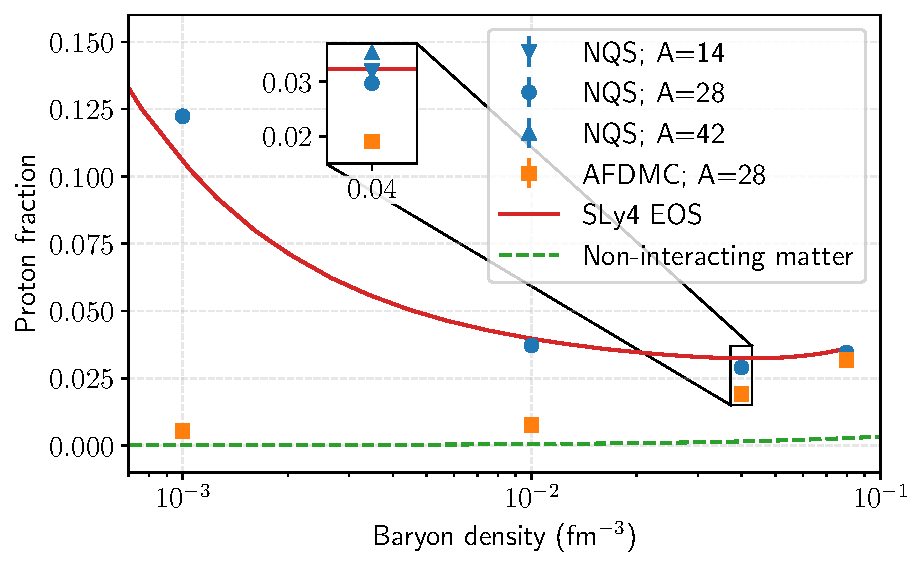
\includegraphics[width=0.7\columnwidth]{figures/nuclear_matter/BEM_proton_fraction.pdf}
\caption{Proton fraction in beta-equilibrated matter as a function of baryon density. Blue circles and orange squares represent NQS and AFDMC calculations for $A=28$ nucleons, respectively. Blue up-triangles and down-triangles indicate NQS results for $A=42$ and $A=14$, respectively, highlighting finite-size effects. The green dashed line shows non-interacting matter, and the red solid curve represents a Skyrme parametrization of the equation of state (SLy4 EOS) for the inner crust of neutron stars~\cite{chabanat1998, douchin2001}. The inset displays NQS results for varying particle numbers at a density of 0.04 fm$^{-3}$ to illustrate finite-size effects.}
\label{fig:x_vs_rho}
\end{figure}



\subsection{Electroweak interactions}
\label{sub:electroweak}
Studying the response of a many-body system to perturbative probes is of great relevance for extracting information about the system’s dynamical structure at both the nuclear and nucleon levels~\cite{bacca_electromagnetic_2014}. These calculations are crucial for interpreting electron-scattering experiments, including assessing whether explicit QCD effects are required to explain the measured response functions~\cite{lovato_charge_2013,cloet_relativistic_2016,lovato_electromagnetic_2016}. Moreover, they are essential for fully exploiting current and next-generation accelerator-based neutrino oscillation experiments~\cite{lovato_ab_2020,acharya_16o_2024}, which use atomic nuclei in their detectors to enhance event rates.

In the linear-response regime, the interaction of an atomic nucleus with electroweak probes is described by the nuclear response function
\begin{equation}\label{eq:resp}
  {\cal R}(\omega)=\sumint_f |\langle\Psi_f | \hat O | \Psi_0 \rangle |^2 \delta{(E_f-E_0-\omega)} \,,
\end{equation}
which encapsulates the dynamical part of the reaction.
In the above equation, \( \hat O \) denotes the excitation operator, while
\( \lvert \Psi_0 \rangle \) and \( \lvert \Psi_f \rangle \) represent the initial and final
states of the system, with energies \( E_0 \) and \( E_f \), respectively.
The final state may be either bound (belonging to the discrete part of the spectrum)
or unbound (in the continuum).
A direct evaluation of the response function therefore, in principle,
requires calculating each individual transition amplitude.

Microscopically computing continuum wave functions for medium-mass nuclei remains an outstanding theoretical challenge. At each continuum energy, the many-body wave function fragments into numerous channels, each representing a distinct breakup configuration, leading to substantial complexity in both momentum and coordinate representations. Integral transform techniques, such as the Laplace transform~\cite{carlson_euclidean_1992} and the Lorentz integral transform (LIT)~\cite{efros_lorentz_2007}, circumvent the difficulties associated with the direct calculation of continuum final states, reformulating the problem as a bound-state calculation. 

The LIT is defined as
\begin{equation} \label{LIT}
  {\cal L}(\omega_0,\Gamma)=\int_{\omega_{th}}^\infty d\omega
  \frac{{\cal R}(\omega)}{(\omega-\omega_0)^2+\Gamma^2}\,,
\end{equation}
where \( \omega_{th} \) is the threshold energy and \( \Gamma>0 \) is the Lorentzian width, serving as a resolution parameter. The LIT method proceeds in two steps. First, \( {\cal L}(\omega_0,\Gamma) \) is computed directly, without requiring explicit knowledge of \( {\cal R}(\omega) \). In a second step, the dynamical response function is obtained through an inversion of the LIT.
 

The function ${\cal L}(\omega_0,\Gamma)$ can be computed starting from its definition and substituting the expression in Eq.~\eqref{eq:resp} for ${\cal R}(\omega)$. Using the completeness relation of the Hamiltonian eigenstates 
\begin{equation}
\sumint_f | \Psi_f \rangle \langle \Psi_f | =1 
\end{equation}
yields 
\begin{align}
{\cal L}(\omega_0,\Gamma)=\frac{\Gamma}{\pi} \langle \Psi_0|{ \hat O}^\dagger \frac{1}{( \hat H - z) } \frac{1}{(\hat H - z^\ast)} \hat O |\Psi_0 \rangle\, .
\end{align}
We denote with $\Psi_L$ the solution of the inhomogeneous  Schr\"odinger equation
\begin{equation}\label{psiL}
( \hat H - z) |\Psi_L\rangle = \hat O | \Psi_0 \rangle \;,
\end{equation}
where \(z = E_0 + \omega_0 + i\Gamma\). Finding the solution for different values of $\omega_0$ and $\Gamma$ lead directly to the transform
\begin{equation}
{\cal L}(z)= \frac{\Gamma}{\pi}\langle \Psi_L |\Psi_L\rangle\, .
\end{equation}
Because ${\cal L}(z)$ is finite, the solution of Eq.~\eqref{psiL} has the same asymptotic boundary conditions as a bound state.

In Ref.~\cite{parnes_nuclear_2026}, the LIT of the dipole operator was computed for the first time using NQS, specifically the Pfaffian--Jastrow ansatz of Eq.~\eqref{eq:pf_even}, to represent both \( \Psi_0 \) and the LIT state \( \Psi_L \). In that work, the LIT equation is solved by maximizing the quantum fidelity between the auxiliary state
\( \lvert \Psi \rangle \equiv (\hat H - z)\lvert \Psi_L \rangle \)
and the source state
\( \lvert \Phi \rangle \equiv \hat O \lvert \Psi_0 \rangle \),
where the fidelity is defined as~\cite{sinibaldi_unbiasing_2023}
\begin{equation}
\mathcal{F}(\Psi, \Phi) =
\frac{\langle \Psi | \Phi \rangle \langle \Phi | \Psi \rangle}
{\langle \Psi | \Psi \rangle \langle \Phi | \Phi \rangle}\,.
\end{equation}
The optimal parameters $\params$ of the NQS are obtained by maximizing a linear combination of the fidelity defined above and a reverse Kullback--Leibler divergence between the target and proposal distributions $\mathrm{KL}\!\left(\pi_{\Psi}\,\|\,\pi_\Phi\right)$,
where 
\begin{equation}
\pi_{\Psi}(X)=\frac{|\Psi(X)|^2}{\langle\Psi|\Psi\rangle}\quad , \quad \pi_\Phi(X)=\frac{|\Phi(X)|^2}{\langle\Phi|\Phi\rangle}\, .
\end{equation}
The gradient of the loss function reads
\begin{equation}
g_{\params}=\nabla_{\params}\mathcal{F}
-\lambda\,\nabla_{\params}\mathrm{KL}\!\left(\pi_{\Psi}\,\|\,\pi_\Phi\right)\,,
\end{equation}
with \( \lambda=1 \) in typical applications.
Stable parameter updates are achieved by employing the \textsc{spring} algorithm (see Section~\ref{subsec:opt})~\cite{goldshlager_kaczmarz-inspired_2024}, which leads to the damped linear system
\(
\bigl(S+\epsilon I\bigr)\delta{\params}
=g_{\params}+\epsilon\,\mu\,\delta{\params}_{\text{prev}}\,.
\)
To ensure scale invariance, the authors of Ref.~\cite{parnes_nuclear_2026} set \( \epsilon=\varepsilon\langle\mathrm{diag}(S)\rangle \)
with a small \( \varepsilon=10^{-3} \).
Note that maximizing the fidelity only fixes the auxiliary state $|\Psi\rangle$ up to an overall complex normalization constant~\cite{hendry_machine_2019}, given by $\mathcal{N} = \langle \Phi | \Psi\rangle / \langle \Phi | \Phi \rangle$, which is estimated stochastically by sampling from $\pi_{\Phi}(X)$. 

%Note that \( \bar \Psi_L\) and \( \Psi_L \) have a different norm and a phase, e.g. $|\bar{\Psi}_L\rangle \approx \mathcal{N} |\Psi_L\rangle $ ~\cite{hendry_machine_2019} which can not be constrained by maximizing the fidelity. This complex constant is given by $\mathcal{N} = \langle \Phi | \bar{\Psi}\rangle / \langle \Phi | \Phi \rangle$, and the latter ratio is estimated stochastically by sampling from $\pi_{\Phi}(X)$. 





Computing the LIT as the norm of \(\Psi_L\) is computationally challenging due to the slowly decaying and oscillatory tails of this wave function. To address this difficulty, one can rewrite the norm as  
\begin{equation}
\langle\Psi_{L}|\Psi_{L}\rangle=\langle\Phi|\frac{1}{\hat{H}-z^{*}}\frac{1}{\hat{H}-z}|\Phi\rangle\nonumber=\frac{1}{\Gamma}\operatorname{Im}\langle\Phi | \Psi_{L}\rangle
\label{eq:lit_xilin}
\end{equation}
which can instead be estimated in a numerically stable manner by sampling from \( \pi_\Phi(X) = |\Phi(X)|^2 / \langle \Phi | \Phi \rangle \). 
The authors of Ref.~\cite{parnes_nuclear_2026} also provide the following upper bound on the LIT uncertainty
\begin{align}
\Delta\mathcal{L}(\omega_{0},\Gamma) &\leq 
\mathcal{D} \; \frac{\mathcal{N}^{-1}||\Phi\rangle|}{\Gamma} \sqrt{\frac{1 - \mathcal{F}  }{ \mathcal{F} }},
\label{eq:error}
\end{align}
where
\begin{equation}
    \mathcal{D} = \min\Big(
\left|(1 - P_{\Phi})|\Psi_L\rangle\right|,\Big|(1 - P_{\Phi})  \frac{H}{\left|z\right|}|\Psi_L\rangle\Big|
\Big),
\end{equation}
and $P_\Phi=|\Phi\rangle\langle \Phi|/\langle \Phi|\Phi\rangle$. This relation implies that in the limit $\Gamma\to 0$, $\omega_0\approx\omega$, and
${\cal L} \to (\pi/\Gamma) {\cal R}$ one finds $\Delta {\cal L}/{\cal L} \propto \sqrt{(1-{\cal F})/\Gamma}$.
Hence, choosing a smaller $\Gamma$ not only makes the required wave function more complex, but also demands correspondingly higher fidelity in the solution of the LIT equation.

Once the central values and the corresponding uncertainties of the LIT are determined, one needs to invert the 
integral transform to retrieve the response function and obtain the corresponding cross sections to be compared with experimental data. In Ref.~\cite{parnes_nuclear_2026} two different techniques have been investigated. The first is a regularized version of the standard inversion procedure introduced in Ref.~\cite{efros_lorentz_2007}, which relies on a suitable basis expansion of the response function. The second is an improved version of the so-called Bryan's version of the Maximum Entropy method~\cite{jarrell_bayesian_1996} which enables the propagation of the uncertainties in $\mathcal{L}(\omega_0, \Gamma)$ into the reconstructed ${\cal R}(\omega)$ using Bayes' theorem.  

Figure \ref{fig:He4_sigma}, adapted from  Ref.~\cite{parnes_nuclear_2026} displays the photodisintegration cross section of $^4$He, obtained by inverting the LIT computed for $\Gamma = 10$ MeV within the NQS framework, and compare it with experimental data from Ref.~\cite{bacca_electromagnetic_2014}. The basis-expansion inversion method in orange and the maximum entropy approach in blue yield results that agree remarkably well with experiment, despite the simplicity of the input Hamiltonian. 


\begin{figure}[!t]
    \centering
    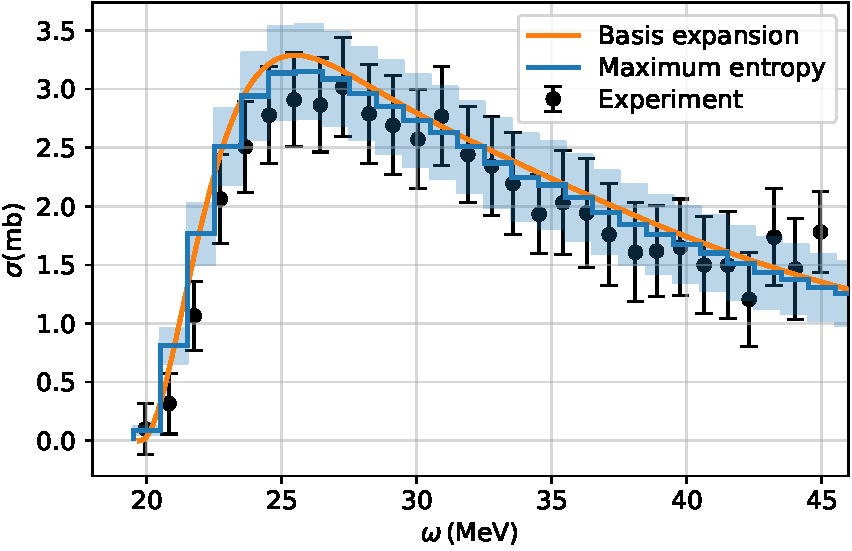
\includegraphics[width=0.5\columnwidth]{figures/applications/he4_sigma.pdf}
    \caption{Adapted from Ref.~\cite{parnes_nuclear_2026} with permission from the Authors. Photo-disintegration cross section of $^4$He as a function of photon energy, obtained from NQS calculations of the LIT. The basis function results (solid orange lines) and the Maximum Entropy reconstruction (blue histogram with error bars) show good agreement with experimental data from Ref.~\cite{bacca_electromagnetic_2014}.}
    \label{fig:He4_sigma}
\end{figure}



\subsection{Pairing interactions and the occupation-number formalism}
\label{sub:pairing}

All $A>2$ nuclear physics applications of NQS discussed so far entail solving the quantum many-body problem in coordinate space, with the antisymmetry of the wave function enforced explicitly through tailored architectures, such as Slater determinants or Pfaffians.
In this setting, fermionic statistics are hard-coded at the level of the wave function ansatz.
A complementary and conceptually distinct approach consists in working in the occupation-number (second-quantized) formalism~\cite{choo_fermionic_2020}, where the many-body basis is built from antisymmetrized Fock states.
In this representation, fermionic antisymmetry is not imposed on the neural-network architecture itself, but is instead automatically taken into account when evaluating expectation values of quantum-mechanical operators through the underlying algebra of creation and annihilation operators~\cite{fetter_quantum_2012}.
This shifts the burden of enforcing antisymmetry from the variational ansatz to the operator formalism.

In the second quantization setting within the occupation number formalism, a NQS representation can be chosen to be
\begin{equation}
\Psi(N) \equiv \langle N | \Psi \rangle\,,
\end{equation}
where $|N\rangle = |n_1,\dots,n_P\rangle$ denotes a basis state in Fock space. The state is specified by occupation numbers $n_i$ indicating whether the fermionic mode $i$ is occupied ($n_i=1$) or empty ($n_i=0$).
Within this general framework, a particularly important class of applications involves pairing correlations, which provide a natural setting for occupation-number--based NQS approaches.
In many physically relevant applications, the full fermionic Fock space is further restricted to a subspace adapted to the dominant correlations of the problem.
For pairing interactions, this corresponds to limiting the Hilbert space to seniority-zero configurations, in which fermions occupy time-reversed states in correlated pairs.
Within this restricted subspace, the occupation-number representation naturally encodes the presence or absence of fermion pairs in a set of active modes.

From a physical perspective, pairing correlations underlie a wide range of phenomena in interacting fermionic systems~\cite{bohr_possible_1958,ring_nuclear_1980,dean_pairing_2003}.
BCS theory provides the canonical framework for understanding pairing in electronic superconductors, wherein fermions near the Fermi surface form correlated Cooper pairs, giving rise to superconductivity.
Soon after the formulation of BCS theory, Bohr, Mottelson, and Pines identified an analogous pairing mechanism in atomic nuclei, in which nucleons near the Fermi surface form spin-singlet pairs~\cite{bohr_possible_1958}.

In finite nuclei, pairing manifests itself through characteristic signatures such as enhanced binding of even--even systems, energy gaps to the first excited states, and systematic trends in excitation spectra and moments of inertia.
These effects are commonly described within mean-field frameworks such as BCS and its particle-number conserving extensions, most notably the Hartree--Fock--Bogoliubov formalism~\cite{dobaczewski_pairing_2001}.
Beyond the mean-field level, symmetry restoration and configuration mixing techniques further refine the treatment of pairing correlations, particularly in finite systems.

Pairing Hamiltonians also play an important methodological role.
Despite their apparent simplicity, they capture essential nonperturbative physics and include integrable subclasses, such as the Richardson--Gaudin models~\cite{richardson_restricted_1963,richardson_application_1963,gaudin_diagonalisation_1976}, which admit essentially exact solutions.
As a result, pairing models provide valuable benchmarks for many-body methods, allowing controlled assessments of accuracy across weak- and strong-coupling regimes.

In its most compact form, the pairing Hamiltonian proposed by Richardson is given by
\begin{equation}\label{eq:pairing_ham}
H = \sum_{p=1}^P d_p N_p - \sum_{p, q = 1}^P g_{pq} A_p^\dagger A_q,
\end{equation}
where $N_p = \sum_{\sigma \in \{\minus, \plus\}} a_{p \sigma}^\dagger a_{p \sigma}$ is the pair number operator.
The operators $A_p^\dagger = a_{p\plus}^\dagger a_{p\minus}^\dagger$ and $A_p = a_{p\plus} a_{p\minus}$ create and annihilate fermion pairs, respectively.
Exact solutions for this model can be obtained both for uniform pairing strengths, $g_{pq} = g$ for all $p,q = 1,\ldots,P$, and for separable hyperbolic couplings of the form
$g_{pq} = 2g\,\sqrt{(\alpha - d_p)(\alpha - d_q)}$.

Once a neural-network quantum-state ansatz $\Psi_V(N)$ is adopted to represent the many-body wave function, quantum-mechanical expectation values can be estimated stochastically using the Metropolis--Hastings algorithm.
Since the number of fermion pairs is conserved, admissible Monte Carlo updates consist of exchanging occupations between pair modes, ensuring ergodicity of the sampling.
This procedure is directly analogous to the isospin-exchange moves discussed in Section~\ref{sec:nqs} within the first-quantized formulation.

As in coordinate-space approaches, the optimal values of the variational parameters defining the NQS are determined by invoking the variational principle.
To this end, all optimization strategies introduced in Section~\ref{sec:nqs} remain applicable in the occupation-number representation, including the stochastic reconfiguration method supplemented with the RMSProp-inspired shift of Eq.~\eqref{eq:sr_rmsprop}.

The main advantage of this formalism is that the NQS itself does not need to be antisymmetric.
As a result, relatively simple architectures, such as restricted Boltzmann machines and feed-forward neural networks, provide valid representations of the many-body wave function (see however Refs.~\cite{passetti_can_2023,denis_comment_2025} for a critical assessment of the representational power of NQS in second quantization).
To demonstrate the power of this approach, the authors of Ref.~\cite{rigo_solving_2023} consider the pairing Hamiltonian in Eq.~\eqref{eq:pairing_ham} for the exactly solvable uniform-coupling and separable-coupling cases. The NQS is parameterized as
\begin{equation}
    \Psi_V(N) = e^{\mathcal{U}(N)} \tanh \big[ \mathcal{V}(N) \big],
\end{equation}
where both $\mathcal{U}(N)$ and $\mathcal{V}(N)$ are MLPs. Although this functional form resembles those employed in Refs.~\cite{adams_variational_2021,gnech_calculation_2020,yang_consistent_2022}, the resulting architectures are significantly simpler, as they do not rely on permutation-invariant Deep Sets constructions~\cite{fuchs_deepsets_2019}.




\begin{figure}[t]
  \centering
  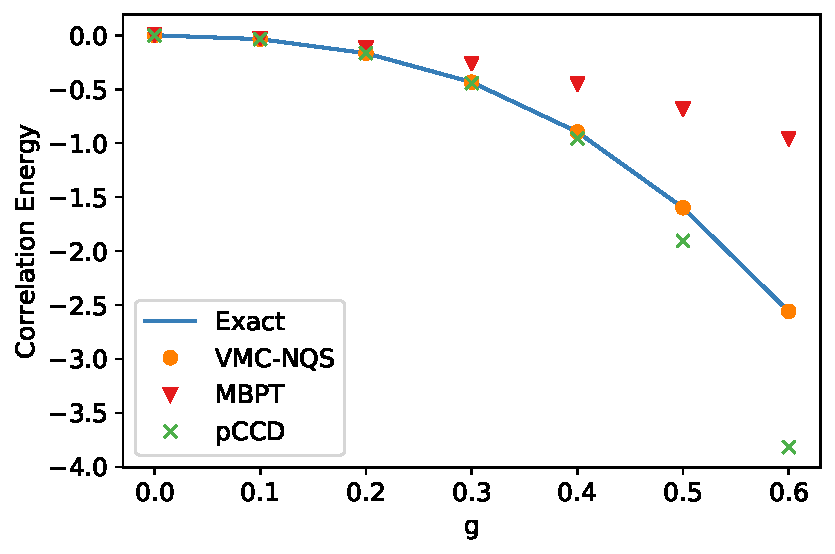
\includegraphics[width=0.48\textwidth]{figures/pairing/g_constant_energies.pdf}\hfill
  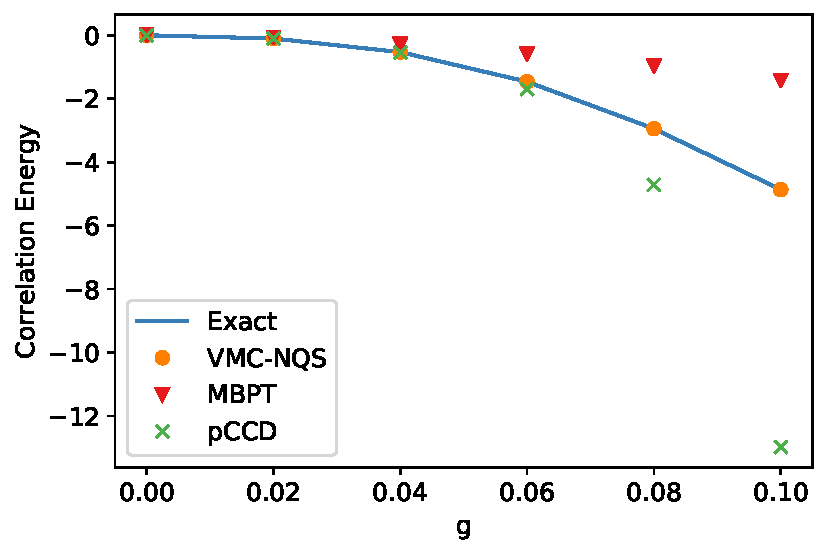
\includegraphics[width=0.48\textwidth]{figures/pairing/g_separable_energies_small.pdf}
  \caption{Correlation energies as a function of the interaction strength $g$ for the constant-coupling pairing model (left) and the separable-coupling model (right), both with $P=10$ energy levels and five fermion pairs.
  Results from VMC-NQS (orange circles), MBPT (red triangles), and pCCD (green crosses) are compared with the exact solution (solid blue line).}
  \label{fig:pairing_side_by_side}
\end{figure}


In Fig.~\ref{fig:pairing_side_by_side}, Ref.~\cite{rigo_solving_2023} compares correlation energies obtained with VMC--NQS, many-body perturbation theory (MBPT), and pair coupled-cluster doubles (pCCD) against the exact solution for both the constant-coupling and separable-coupling pairing models.
While all approaches yield similar results in the weak-coupling regime, MBPT rapidly deviates from the exact solution as the interaction strength increases, reflecting the breakdown of perturbation theory in the presence of strong pairing correlations.
The pCCD method exhibits a different failure mode, significantly overbinding at intermediate and strong coupling and thereby violating the variational principle, with particularly pronounced deviations for the separable interaction.
In contrast, the VMC--NQS results closely track the exact correlation energies across the entire range of coupling strengths shown, remaining accurate deep into the non-perturbative regime.
Taken together, these results demonstrate that occupation-number--based NQS provide a highly accurate and variationally controlled description of pairing Hamiltonians, successfully capturing collective correlations across weak- and strong-coupling regimes where conventional many-body methods fail.

At the same time, this success must be understood within the scope of the models considered.
When pairing Hamiltonians are formulated in terms of an underlying single-particle basis, realistic nuclear interactions are strongly non-perturbative.
Converged calculations therefore require a large number of single-particle orbitals.
Consequently, the dimension of the single-particle basis typically satisfies $P \gg A$, where $A$ is the number of nucleons.
In state-of-the-art no-core shell-model calculations~\cite{barrett_ab_2013}, $P$ can reach several thousand.
This, in turn, leads to neural-network representations of prohibitive size.
As a result, the applicability of occupation-number--based NQS approaches to fully realistic nuclear Hamiltonians remains limited at present, motivating the exploration of complementary representations and hybrid strategies.





%

Pairing lies at the heart of nuclear physics and the quantum
many-body problem in general \cite{ring_nuclear_1980,richardson_restricted_1963,dean_pairing_2003}.
Pairing correlations, the tendency of identical nucleons to form correlated Cooper pairs, play an important role in  nuclear many-body systems.  Soon after the Bardeen–Cooper–Schrieffer (BCS) theory explained electron superconductivity, Bohr, Mottelson, and Pines famously pointed out an analogy in nuclei, namely that nucleons near the Fermi surface couple into Cooper pairs, giving rise to nuclear superfluidity~\cite{bohr_possible_1958}.  Early applications of BCS theory to nuclei demonstrated that including pairing dramatically improves the description of nuclear properties. Indeed, pairing underlies numerous phenomena in finite nuclei, from the extra binding of even-even nuclei to their characteristic excitation spectra. 

In nuclear physics, pairing is treated using models originally inspired by electronic superconductors. The simplest approach is the BCS model \cite{richardson_restricted_1963,bohr_possible_1958}, in which a condensate of nucleon pairs (typically in a spin-singlet, $^1S_0$ state) occupies the nuclear ground state. The BCS theory successfully explained why even-even nuclei are more tightly bound than their odd-$A$ neighbors (the odd–even mass staggering) and why even-even nuclei have an energy gap to the first excited state. However, the standard BCS wave function is not an eigenstate of particle number and it violates the conservation of nucleon number by allowing coherent superpositions of different particle numbers. In the mean-field context, this is remedied by the Hartree–Fock–Bogoliubov (HFB) approach \cite{Dobaczewski2002}, which combines the Hartree–Fock description of single-particle motion with a Bogoliubov transformation to incorporate pairing correlations self-consistently. This approach extends the independent-particle model to a quasiparticle basis, wherein the normal single-particle density and the pairing tensor are determined simultaneously by variational minimization of the energy. This formalism (and its variants within energy density functional theory) is the workhorse for modeling open-shell nuclei and has been applied extensively across the nuclear chart and even to uniform nuclear matter . For example, HFB calculations with effective interactions can predict pairing gaps in nuclei and in neutron-star matter within a unified framework.

Beyond the mean-field level, important refinements to pairing theory have been developed. One class of methods focuses on restoring broken symmetries – in particular, enforcing exact particle-number conservation. 

In finite nuclei, pairing correlations profoundly shape nuclear structure. A primary signature is the odd–even staggering of binding energies: nuclei with an even number of neutrons (and/or protons) are systematically more bound than the interpolating odd-$A$ nuclei, reflecting the energy gain from pairing two like nucleons. Quantitatively, this pairing gap is on the order of $\sim1$–2 MeV in many medium and heavy nuclei, see for example \cite{Dean2003} for examples. Even–even nuclei (with all nucleons paired) exhibit a pairing gap in their excitation spectrum. Here, the lowest excited state requires breaking a Cooper pair. In contrast, neighboring odd-$A$ nuclei (with one unpaired nucleon) have a compressed low-lying spectrum, as the unpaired quasiparticle can be excited with much smaller energy. These differences are borne out in experiments across the nuclear chart and are classic evidence of pairing correlations in nuclei. Likewise, the structure of nuclear shells is expected to be affected  by pairing correlations. At magic numbers, pairing is suppressed by the large single-particle energy gap, leading to reduced odd–even staggering, whereas for open-shell nuclei pairing correlations  smooth out many irregularities in nuclear masses.
Thus, many observable quantities such as  the magnitude of odd–even mass differences, the excitation energy of the first $2^+$ state in even-even nuclei, or the moment of inertia of rotational bands etc., serve as benchmarks for theoretical pairing models.


Pairing is not only a finite-nucleus phenomenon, it also plays a key role in infinite nuclear matter, particularly in the extreme environment of neutron stars. In the dense interior of neutron stars, nucleons are believed to form Cooper pairs and undergo a transition to superfluid (neutron) and superconducting (proton) phases at temperatures of order $10^9$–$10^{10}$ K (about $0.1$–1 MeV) \cite{Dean2003}.


Thus, pairing correlations are a central ingredient in effective nuclear
interactions and strongly influence ground-state energies and
low-energy structure. Furthermore, the pairing Hamiltonian is also an attractive
methodological testbed. It is nontrivial, yet possesses integrable
subclasses (Richardson-Gaudin models) \cite{Gaudin:1976} that provide essentially exact
benchmarks. The aim of this part of the present review is to
demonstrate that a \emph{variational}, neural-network-based solver,
with a discrete single-particle basis as used in typical nuclear
shell-model diagonalization approaches, can reproduce near-exact
correlation energies across weak and strong coupling regimes in a way
that remains reliable when common approximations such as
many-body-perturbation theory \cite{Paldus2006,shavittbartlett2009,morten_book} 
and coupled-cluster theory \cite{shavittbartlett2009,Hagen:2013nca} start
deviating from benchmark results from Full Configuration Interaction (FCI)
theory. Furthermore, this excursion into neural network calculations
in a discrete single-particle basis and effective Hamiltonians,
demonstrate the broad range of applicabilities of our deep learning
methods. The results presented here are all taken from Ref.~\cite{rigo2023}.



Our specific model consists of a total of $P$ doubly degenerate and equally spaced
single-particle levels labelled by $p=1,2,\dots$ and spin $\sigma=\pm
1$.  These states are schematically portrayed in
Fig.~\ref{fig:schematic}.  
The $P$ doubly-degenerate single-particle levels are occupied by $M$ time-reversed fermion pairs. In the usual
second-quantized form, the Hamiltonian is written as
\begin{equation}
H=\sum_{p,\sigma} d_p\, a_{p\sigma}^\dagger a_{p\sigma}
-\sum_{p,q} g_{pq}\, a_{p+}^\dagger a_{p-}^\dagger a_{q-} a_{q+},
\label{eq:H_full}
\end{equation}
with $d_p$ the single-particle energies and $g_{pq}$ the pairing matrix elements. 
In the expressions below we will find it useful to introduce rhe pair operators $A_p^\dagger=a_{p+}^\dagger a_{p-}^\dagger$ and $A_p=a_{p-}a_{p+}$ and the pair-number operator
$N_p=\sum_{\sigma}a_{p\sigma}^\dagger a_{p\sigma}$.



The interaction can only couple pairs and excites therefore only two
particles at the time, as indicated by the rightmost four-particle
state in Fig.~\ref{fig:schematic}. There, a pair is excited to the
state with $p=9$.   

In our model we have kept both the interaction strength and the single-particle level as constants.
In a realistic system like a nucleus, this is not the case; however, if a harmonic oscillator basis
is used, at least the single-particle
basis mimicks the input to realistic effective interactions in nuclear physics calculations.  

\begin{figure}[hbtp]
    \centering
    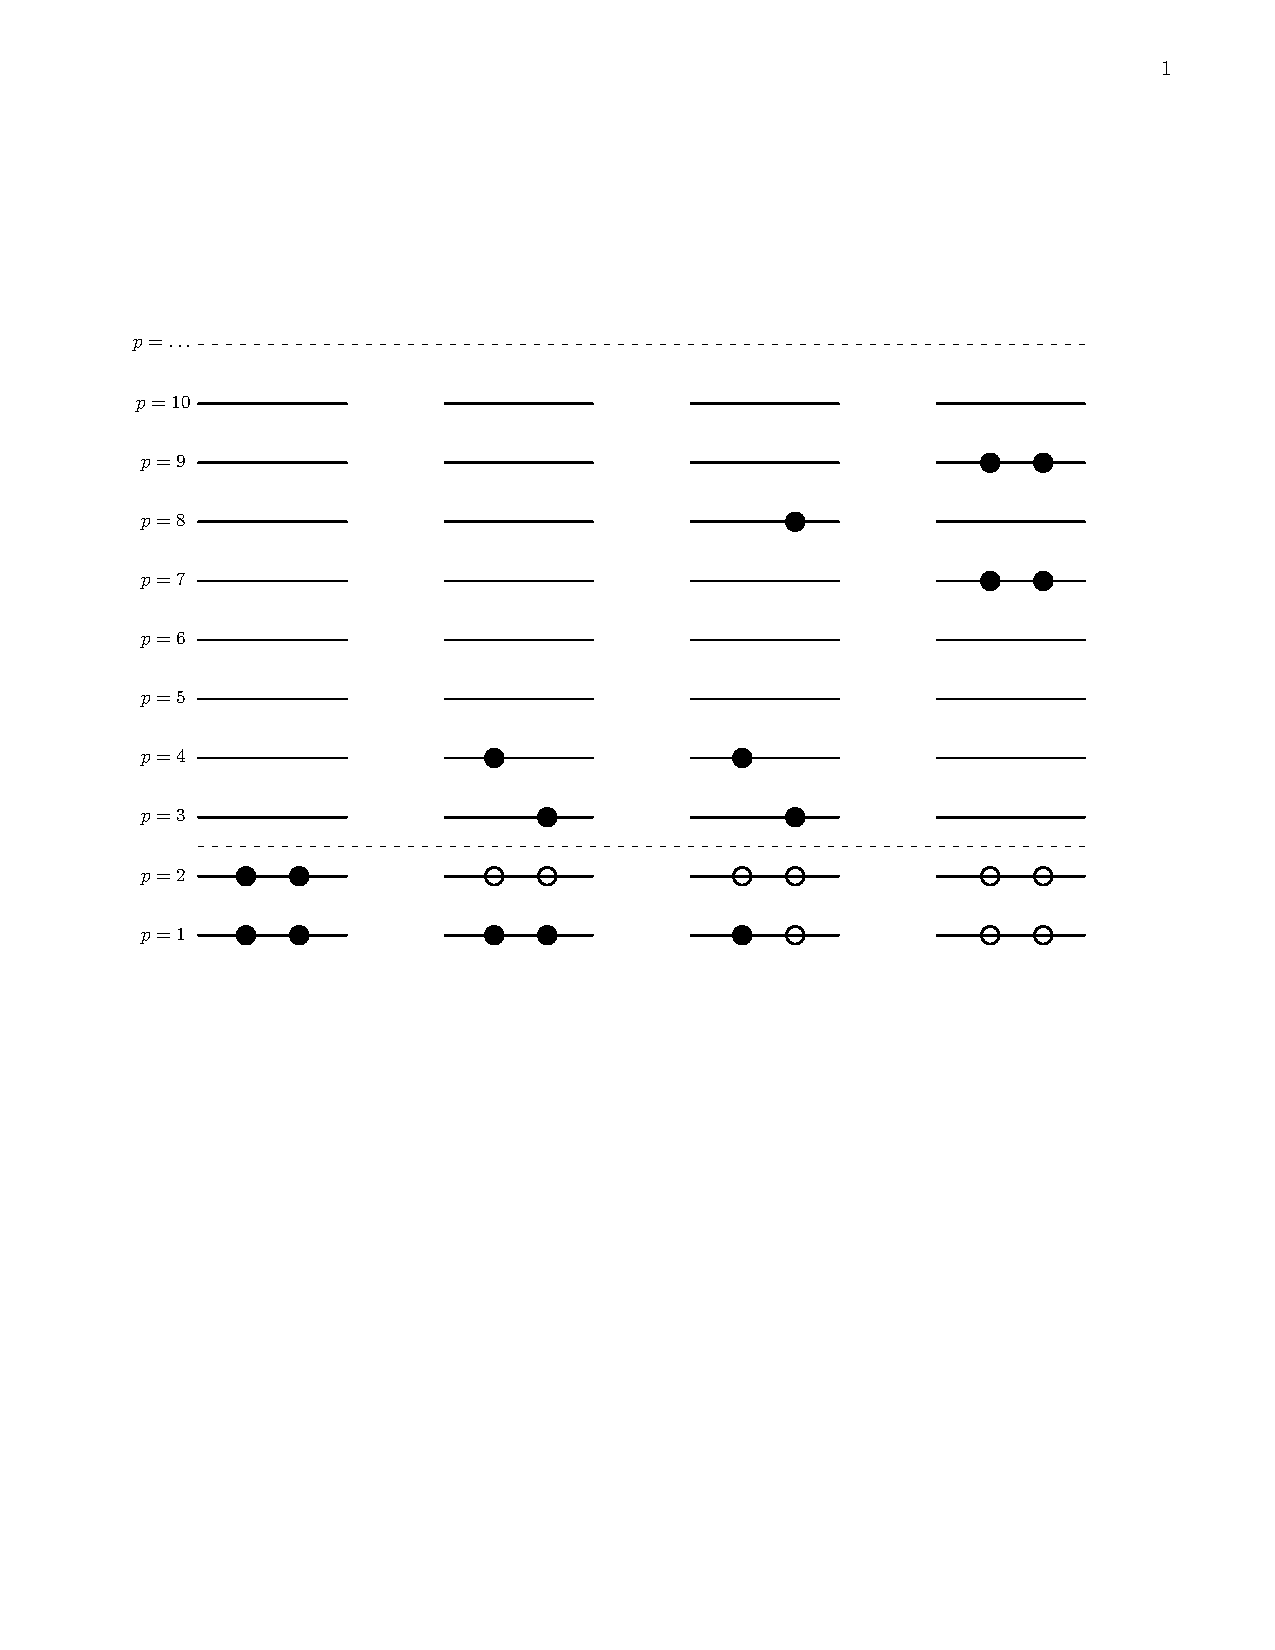
\includegraphics[width=0.7\textwidth]{figures/pairing/figpairing.pdf}
  \caption{Schematic plot of the possible single-particle levels with double degeneracy for four fermions.
The filled circles indicate occupied particle states while the empty circles 
represent vacant particle(hole) states.
The spacing between each level $p$ is constant in this picture. 
The first state to the left represents
a possible ground state representation for a four-fermion system. In the second state to the left,
one pair is broken by the interaction. 
All single-particle orbits belong to the model space. The two remaining four-particle states represents single-particle excitations to the excluded space, either by breaking two pairs or breaking one pair and exciting one pair (rightmost state). The latter two configurations cannot be produced by the pairing interaction alone. One would need to add an explicit pair-breaking term to the Hamiltonian.\label{fig:schematic}}
\end{figure}

Two exactly solvable cases play a central role in the benchmarks discussed in \cite{rigo2023} and reviewed here.
We distinguish between a so-called
\textbf{Constant-coupling pairing} with $g_{pq}=g$, giving
\begin{equation}
H=\sum_{p=1}^P d_p N_p - g\sum_{p,q=1}^P A_p^\dagger A_q,
\label{eq:H_const}
\end{equation}
with ground-state energies obtainable from Richardson equations \cite{Richardson:1963a,Richardson:1963b} (coupled nonlinear equations for pair energies). The next case is the so-called 
\textbf{Separable (hyperbolic) pairing}, with  a separable interaction with an energy cutoff $\alpha$,
\begin{equation}
H=\sum_{p=1}^P d_p N_p -2g\sum_{p,q=1}^P \sqrt{(\alpha-d_p)(\alpha-d_q)}\,A_p^\dagger A_q,
\label{eq:H_sep}
\end{equation}
which belongs to the hyperbolic Richardson-Gaudin family and is also
solvable by a related set of coupled equations.
These two approaches are used to assess the accuracy of our
network approaches beyond those model-spaces (defined by the
doubly-degenerate single-particle orbits $p$) that can be handled by
FCI theory.

Our variational Monte Carlo approach minimizes the Rayleigh--Ritz variational energy
\begin{equation}
E_V(\bm{\theta})=\frac{\bra{\psi_V(\bm{\theta})}H\ket{\psi_V(\bm{\theta})}}{\langle\psi_V(\bm{\theta})\vert\psi_V(\bm{\theta})\rangle},
\qquad E_0\le E_V(\bm{\theta}),
\label{eq:Ev}
\end{equation}
by varying the parameters $\bm{\theta}$ of a trial state $\ket{\psi_V}$.
In an occupation-number basis $\ket{\bm{n}}$ (here $\bm{n}=(n_1,\dots,n_p)$ with $n_p\in\{0,1\}$ indicating whether
a \emph{pair} occupies level $p$), the variational amplitudes are $\psi_V(\bm{n})=\braket{\bm{n}|\psi_V}$.
The configurations are sampled from
\begin{equation}
\mathbb{P}(\bm{n})\propto \vert\psi_V(\bm{n})\vert^2,
\label{eq:prob}
\end{equation}
and the energy estimator uses the local energy $E_L(\bm{n})$.
A practical advantage is that the occupation-number representation automatically encodes
fermionic antisymmetry/Pauli constraints, allowing comparatively simple NQS architectures. 
Our neural-network quantum state ansatz employs a real-valued NQS of the form
\begin{equation}
\psi_V(\bm{n})=e^{U(\bm{n})}\tanh\!\big(V(\bm{n})\big),
\label{eq:nqs}
\end{equation}
where $U$ and $V$ are fully connected feed-forward networks. In this parametrization, $U$ controls the magnitude,
while $\tanh(V)$ provides a smooth representation of the sign structure. In Ref.~\cite{rigo2023}, the author typically used two to three  hidden layers with
the $\tanh$-function as  activation function for the hidden layers. 

In the pairing Hamiltonian, off-diagonal contributions correspond to
moving a pair from an occupied level to an unoccupied one. For a given
configuration $\bm{n}$, only indices with $n_p=1$ and $n_q=0$
contribute, and the needed matrix elements can be computed by looping
over occupied/unoccupied sets and evaluating $\psi_V$ on the
configuration with $n_p\!\to 0$ and $n_q\!\to 1$. This structure keeps
the Monte Carlo evaluation efficient and explicitly tied to the
physical pair-scattering processes.

To optimize $\bm{\theta}$, stochastic reconfiguration  \cite{Sorella:2005} was applied, that is
\begin{equation}
S\,\delta\bm{\theta}=-\delta\tau\,\bm{G},
\label{eq:sr}
\end{equation}
where $\delta\tau$ is a step size, $S$ is an overlap/covariance matrix
of log-derivatives, and $\bm{G}$ is the energy gradient
estimator. Since the number of parameters grows with system size,
explicitly storing $S$ becomes prohibitive; we therefore solve
\eqref{eq:sr} with conjugate gradients, requiring only an efficient
routine for matrix-vector products $S\bm{v}$. To improve stability,
Rigo {\em et al.,} \cite{rigo2023} introduced a small diagonal
regularization inspired by RMSProp/Adam-style second-moment tracking
(with typical diagonal-shift strengths, see \cite{rigo2023} for additional information).

We have here, as done in Ref.~\cite{rigo2023}, chosen to present \emph{correlation energies} and benchmark the VMC--NQS method against exact diagonalization
(where feasible) and against two widely used approximations: many-body perturbation theory (MBPT) and pair coupled
cluster doubles excitations (pCCD). 

Figure \ref{fig:corr_constant} demonstrates the optimization dynamics for the constant-coupling pairing Hamiltonian
\eqref{eq:H_const} with $P=10$ levels and $M=5$ pairs. The plotted observable is the correlation energy
as function of the strength of the pairing interaction.
\begin{figure}[hbtp]
    \centering
    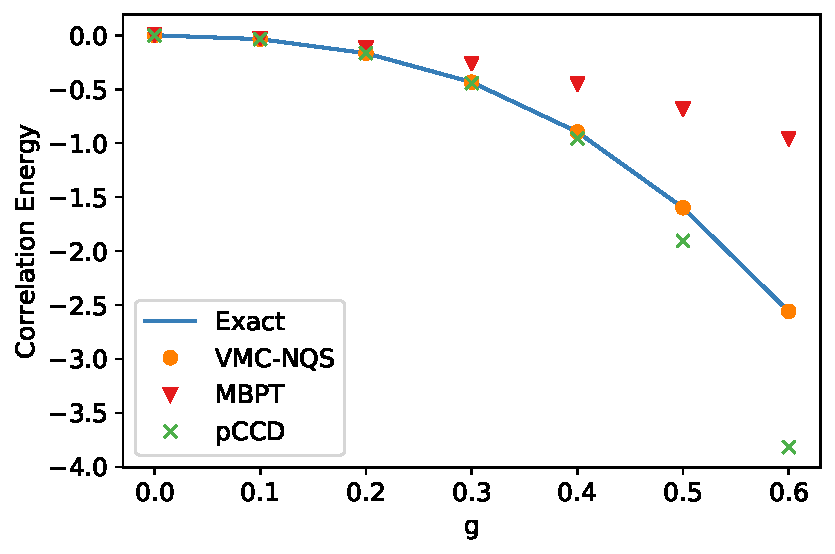
\includegraphics[width=0.8\textwidth]{figures/pairing/g_constant_energies.pdf}
    \caption{Correlation energy for the constant-coupling model for $P=10$ single-particle energy levels and $M=5$ pairs as a function of the interaction strength. VMC-NQS (solid orange circles), MBPT (solid red triangles), and pCCD (green crosses) calculations are compared with the exact answer (solid line). Taken from \cite{rigo2023}.}
    \label{fig:corr_constant}
\end{figure}
After roughly $10^3$ optimization steps, the VMC--NQS correlation energy converges to the exact-diagonalization
value. the final precision level is around $10^{-7}$ in the converged correlation energy.
In this figure, three approximations (MBPT, pCCD, VMC--NQS) are plotted against the exact
result. We note from this figure that 
\begin{itemize}
\item \textbf{Weak coupling:} all methods agree closely at small $\vert g\vert$, consistent with perturbative expectations. 
\item \textbf{MBPT breakdown:} deviations from exact diagonalization become visible already around $g\approx \vert 0.2\vert$. This is interpreted as the inability of low-order perturbation theory to capture
nonperturbative pairing correlations at stronger coupling. 
\item \textbf{pCCD: initially robust, then overbinding:} pCCD remains closer down to about $g\approx \vert 0.4\vert$ but becomes
significantly \emph{too low} for more negative $g$, that is it overbinds and thereby violates the variational principle.
\item \textbf{VMC--NQS: uniform accuracy and variational safety:} VMC--NQS tracks the exact curve across the full range
shown, with discrepancies remaining below $10^{-4}$.
\end{itemize}

The main methodological message of Fig.~\ref{fig:corr_constant} is
that enforcing a \emph{variational} optimization over a flexible NQS
ansatz yields a solver that remains reliable precisely where MBPT and
pCCD lose quantitative control.


The authors of Ref.~\cite{rigo2023}  extended the comparative analysis by considering a larger model
space, with up to $P=40$ energy levels and $M=20$ pairs of
fermions. In Table~\ref{tab:g_constant_large}, we list here  the
correlation energies obtained within VMC-NQS, pCCD, and the
highly-accurate iterative approach for solving the Richardson
equations developed in Ref.~\cite{Guan:2022CoPhC}. To make contact
with the results of the latter reference, the single-particle energies
are re-scaled as $d_p = p / 10$ and the pairing strength is taken to
be $g=-0.05$. Similarly to the smaller model space, the correlation
energies computed within VMC-NQS are almost always in perfect
agreement with the ones obtained from the Iterative method. The only
exception is the case with $P=40$ and $M=20$, for which the VMC-NQS
yields $-1.785$, while the iterative method provides $-2.111$.  On
the other hand, pCCD struggles already for $P=10$ and $M=5$, where it
yields $\sim 20\%$ overbinding. Increasing the number of
single-particle states and pairs, pCCD becomes more and more
unreliable, with large departures from both the exact and VMC-NQS
values. This behavior is due to the the pairing interaction terms
growing faster with the number of states than the mean-field one,
making the exact ground-state very different from the Hartree-Fock
solution.

\begin{table}[hbtp]
\begin{center}
\vspace{0.5cm}
\begin{tabular}{ c | c | c c c c }
\hline
\hline
& $P$ & $M=5$  & $M=10$ & $M=15$ & $M=20$ \\
\hline
VMC-NQS & \multirow{3}{*}{ 10 }  & -0.160 & 0.000 & - & - \\
pCCD &  & -0.193 & 0.000 & - &  -\\
Iterative &  & -0.160  & 0.000 & - & - \\
\hline
VMC-NQS & \multirow{3}{*}{ 20 }  & -0.394 & -0.515 & -0.394 & 0.000 \\
pCCD &   & -0.987 & -1.743 & -1.110 &  0.000 \\
Iterative &   & -0.394 & -0.515 & -0.394 &  0.000 \\
\hline
VMC-NQS & \multirow{3}{*}{ 30 }  & -0.606 & -0.946 & -1.057 & -0.946 \\
pCCD &   & -1.750 & 3.500 & -6.467 &  -5.697\\
Iterative &   & -0.606 & -0.946 & -1.057 & -0.946\\
\hline
VMC-NQS & \multirow{3}{*}{ 40 }  & -0.809 & -1.356 & -1.678 & -1.785 \\
pCCD &   & -4.231 & 124.923 & 7.598 &  -44.346 \\
Iterative &   & -0.809 & -1.356 & -1.678 & -2.110\\
\hline
\end{tabular}
\caption{Correlation energies obtained with the VMC-NQS method compared with pCCD and the iterative approach of Ref.~\cite{Guan:2022CoPhC} for the constant-coupling Hamiltonian of Eq.~\eqref{pairing_model_hamiltonian_constant_g} with $g = 0.05$ and $d_p=p/10$. Taken from Ref.~\cite{rigo2023}.}
\label{tab:g_constant_large}
\end{center}
\end{table}

These results establish that a variational Monte Carlo approach  in an occupation-number basis with a
compact NQS ansatz can solve integrable nuclear pairing Hamiltonians
with near-exact accuracy over a wide coupling range, while maintaining
the variational bound by construction. The Stochastic Reconfiguration together with the RMSProp update of the learning rates
provide stable convergence, and the benchmarks against exact
diagonalization show that VMC--NQS remains accurate where MBPT and
pCCD deviate or violate variationality. The authors also report on
broader tests and argue that the approach exhibits polynomial scaling
in $P$, motivating extensions to nonseparable, state-dependent pairing
interactions and to larger shell-model Hamiltonians where exact
diagonalization is infeasible due to too large dimensionalities.







